\documentclass{MScthesisITEM}

% this package is just to generate text for demo-purposes
\usepackage{blindtext}
\usepackage{multirow}
\usepackage{pbox}
\usepackage{csquotes}

\title{International Potential for a Free Model in a B2B\&C market} % The title of your assignement; NB use \newlinetitle to start a newline
\author{Kristian Tagesen} % Your firstname and lastname
\professor{Jan A. Audestad, ITEM} % Affiliation = ITEM for instance
\supervisor{Thomas Jelle, MazeMap}

%% Uncomment the following in case you want subfigures; note that there will be a warning for the caption package
% \let\subcaption\undefined
% \let\subfloat\undefined
% \usepackage[bf]{caption}
% \usepackage{subcaption}

\DeclareGraphicsExtensions{.pdf,.jpg}
\graphicspath{{./figs/}}

\loadglsentries{glossary}
\makeglossaries

\begin{document}
\selectlanguage{english}
\pagenumbering{roman}
\pagestyle{plain}

%% Only for the project; comment out the line below for the master's thesis; the front page will be generated automatically by DAIM
%\titleITEM

%% Only for the master's thesis; for the project report the description is taken from It's Learning and added by the department
 \selectlanguage{english} % Change to 'norsk' if you are writing in Norwegian
 \begin{titlingpage}

\noindent
\begin{tabular}{@{}p{2cm}l}
\textbf{Title:} 	& \thetitle \\
\textbf{Student:}	& \theauthor \\
\end{tabular}

\vspace{4ex}
\noindent\textbf{Problem description:}
\vspace{2ex}

\noindent This thesis will continue the preliminary work done in the report written in the autumn semester of 2015, concerning the potential of the freemium business model in an indoor mapping solution. While the report consisted of a survey that was done nationally, this thesis will expand to include the international market, and will have a narrower scope in that two customer segments will be surveyed. A business model fitting the freemium paradigm will be suggested, and a survey will be presented along with its results. The main goal of the thesis is to try to ascertain whether a freemium model will work in a B2B\&C market, more specifically for an indoor mapping solution.
\vspace{6ex}

\noindent
\begin{tabular}{@{}p{4cm}l}
\textbf{Responsible professor:} 	& \theprofessor \\
\textbf{Supervisor:}			& \thesupervisor \\
\end{tabular}

\end{titlingpage}
 \cleardoublepage

%% There must be an abstract in English, even though the main text is in Norwegian
\selectlanguage{english}
\pagestyle{empty}
\begin{abstract}
\noindent \Blindtext[5][1]
\end{abstract}
\cleardoublepage

%% Only for the master's thesis; if the main text is in English and you can write Norwegian, there must be an abstract in Norwegian as well.
 \selectlanguage{norsk}
 \pagestyle{empty}
\renewcommand{\abstractname}{Sammendrag}
\begin{abstract}
\noindent Sikkerheten til nesten all offentlig nøkkel-kryptografi er basert på et vanskelig beregnbarhetsproblem. Mest velkjent er problemene med å faktorisere heltall i sine primtallsfaktorer, og å beregne diskrete logaritmer i endelige sykliske grupper. I de to siste tiårene, har det imidlertid dukket opp en rekke andre offentlig nøkkel-systemer, som baserer sin sikkerhet på helt andre type problemer. Et lovende forslag, er å basere sikkerheten på vanskeligheten av å løse store likningsett av flervariable polynomlikninger. En stor utfordring ved å designe slike offentlig nøkkel-systemer, er å integrere en effektiv ``falluke'' (trapdoor) inn i likningssettet. En ny tilnærming til dette problemet ble nylig foreslått av Gligoroski m.f., hvor de benytter konseptet om kvasigruppe-strengtransformasjoner (quasigroup string transformations). I denne masteroppgaven beskriver vi en metodikk for å identifisere sterke og svake nøkler i det nylig foreslåtte multivariable offentlig nøkkel-signatursystemet MQQ-SIG, som er basert på denne idéen.

Vi har gjennomført et stort antall eksperimenter, basert på Gröbner basis angrep, for å klassifisere de ulike parametrene som bestemmer nøklene i MQQ-SIG. Våre funn viser at det er store forskjeller i viktigheten av disse parametrene. Metodikken består i en klassifisering av de forskjellige parametrene i systemet, i tillegg til en innføring av konkrete kriterier for hvilke nøkler som bør velges. Videre, har vi identifisert et unødvendig krav i den originale spesifikasjonen, som krevde at kvasigruppene måtte oppfylle et bestemt kriterie. Ved å fjerne denne betingelsen, kan nøkkel-genererings-algoritmen potensielt øke ytelsen med en stor faktor. Basert på alt dette, foreslår vi en ny og forbedret nøkkel-genereringsalgoritme for MQQ-SIG, som vil generere sterkere nøkler og være mer effektiv enn den originale nøkkel-genereringsalgoritmen.  
\end{abstract}
 \cleardoublepage

\selectlanguage{english}% Change to 'norsk' if you are writing in Norwegian

\renewcommand{\abstractname}{Preface}
\begin{abstract}
\noindent This thesis presents my final work and research for my Master of Science degree in Communication Technology at the \gls{ntnu}. I have specialised in ICT economics at the \gls{item}, belonging to the \gls{ime}.
\\
\newline
I wish to extend thanks to my supervisor Thomas Jelle and responsible professor Jan A. Audestad for their everpresent support and valuable input throughout the semester. Furthermore, I wish to thank the respondents of the survey for their contributions, without these answers this thesis could never have been written.

\begin{center}
Kristian Tagesen
\\
Trondheim, June 2016
\end{center}
\end{abstract}
\cleardoublepage

% similarly you may add a separate acknowledgments page

\include{acknowledgments}
\cleardoublepage

\tableofcontents*
\cleardoublepage

%% include if relevant
\listoffigures
\cleardoublepage

%% include if relevant
\listoftables
\cleardoublepage

%% include if relevant
% \listofalgorithms
% \addcontentsline{toc}{chapter}{List of Algorithms}
% \cleardoublepage

%% include if relevant
%\printglossary[title=List of Symbols, style=long]
%\cleardoublepage
%\glsaddall[]

%% include if relevant
\printglossary[title=List of Acronyms,type=\acronymtype] % prints just the list of acronyms
\cleardoublepage

\pagenumbering{arabic}
\pagestyle{ruled}
\chapter{Introduction}
\section{Motivation}

%hvorfor navigasjon er viktig

The indoor mapping service \gls{mm} started as a venture from Wireless Trondheim, an R\&D company working closely (and cooperating) with \gls{ntnu}, and whose goal it is to create sustainable ventures from new ideas. MazeMap's main service is providing an indoor mapping service aimed at large institutions such as universities, hospitals, conference venues, shopping malls and more. Users are able to access the service on any computer, tablet or smartphone, where the indoor maps themselves is the focal point. Navigation services are also available in many different forms, but using Wi-Fi is a readily available and easily deployed solution which has been co-developed with Cisco. This particular service uses a technique called trilateration~\cite{BiczokMJK14}, and is easily implemented as it uses existing Wi-Fi infrastructure to facilitate the service.


\gls{mm} has a very scalable technical platform, in which a robust indoor-map-creating engine resides. The engine is able to convert digital floorplans into full-scale, digital indoor maps that can be accessed from any device capable of running \gls{mm}'s software. Because of its scalable nature, the time needed per customer is low, and little involvement in the setup phase is needed from \gls{mm}'s perspective. Thus, in order to accelerate customer acquisition, a proposition can be made to change or alter the business model: A freemium model has been detrimental in the success of several start-ups in the consumer market, for example Dropbox, Skype, Waze and Snapchat, but it is interesting to see if this can be applied in a \gls{b2b} or a \gls{b2bc} setting with the same success.


Two market drivers are particularly protruding when it comes to indoor maps:
\begin{itemize}
    \item The demand for indoor orientation as buildings become more numerous and complex.
    \item The Internet of Things and fleet management.
\end{itemize}

As of 2015, one of the world's largest shopping mall by total area is the Dubai Mall in Dubai, UAE~\cite{aleksandarjevtic2015}. With its 1,124,000 square meters of space and around 1,200 shops, it was one of the most visited buildings on the planet in 2011, and as much as 34 million people visited it~\cite{anderson2012evolution}, a number that rose to 80 million in 2014~\cite{marysophia2015}. With establishments of such gargantuan proportions, the inherent need for being able to find different points-of-interest presents itself. One apparent solution to this, is of course an \gls{ims} that may be provided to the customers via a smartphone application or stationary touch screens. As opposed to static maps, a digital interactive map allows for greater customer immersion, while providing more valuable information and improving the overall visitor experience. For establishments, analytical tools may be used to track customers in regards to habits, frequency of visits etc. to improve the offering to visiting clientele. Furthermore, establishments with large areas such as universities and hospitals are able to reduce stress and nervousness among visitors, by employing an \gls{ims} that can be used before a visit to familiarise the environment~\cite{mazemaphosp}. As more buildings are being built and experience internal change, updating static maps several times per year can be an undertaking that is readily mitigated by having digital, adaptable maps.


The Global Standards Initiative on Internet of Things has defined the term \gls{iot} as a \textit{"global infrastructure for the information society, enabling advanced services by interconnecting (physical and virtual) things based on existing and evolving interoperable information and communication technologies."}~\cite{itu2016}. In essence, this means that the physical world can be shaped in a way that improves accuracy and efficiency, while granting potential economic benefits~\cite{friess2013internet}. The \gls{iot} is closely related to the concept of fleet management, which in this case pertains to objects connected to the \gls{iot} that may need to be located on a regular basis. This relates to indoor maps in the sense that as physical objects are connected to the Internet, the location of these objects may be obtained from an \gls{ims}. Hospitals are able to show personnel where an ever-changing border of a clean/dirty zone is, as well as showing where equipment is currently situated. Universities are for example able to show its staff and students where they can find the nearest printer, as opposed to merely providing a textual description of where printers are located. As more physical objects are incorporated into the \gls{iot}, the need for fleet management increases and digital indoor maps may be an effective way to accommodate this need. 

\section{Scope \& Objectives}
In order to achieve the goal of determining the effectiveness and feasibility of a freemium model in an international \gls{b2bc}-market, while proposing a fitting business model, it is necessary to narrow down the aspects considered in this thesis. Furthermore, the aim is also to give the reader a clear and concise overview of the topics discussed.

\subsection{Scope}
MazeMap already serves a large base of customers around the world, with their main bottleneck in expanding further being customer acquisition. As means to remedy this and to accelerate customer acquisition, the freemium model can be proposed. Given \gls{mm}'s robust map-generating-engine, the main focus is shifted away from any technical limitations or inherent flaws on \gls{mm}'s end, and is moved towards the viability of a freemium model. Given the scale of a global survey, the survey presented later in the thesis will focus on an already established customer segment, namely \gls{hei}s. This restriction is in place in order to more specifically target this thesis's goal of proposing a business model and determining if a freemium business model is feasible, rather than exploring new customer segments. 

\subsection{Objectives}
This thesis aims to determine the viability and feasibility of a freemium model in a \gls{b2bc}-market, and to propose an appropriate business model in this particular paradigm. In short the objectives can be described in the following manner:
\begin{enumerate}
    \item Investigate if there is a demand for an \gls{ims} operating under the free model
    \item Discuss and interpret the viability of such a service at an international level
    \item Propose a business model based on the findings and its surrounding discussion
\end{enumerate}
Taking the scope into consideration, this forms the basis of the main research question for this thesis: Is a free model viable as a business model in a \gls{b2bc}-market on an international level, and can this model potentially accelerate customer acquisition?

\section{Contribution}
Mainly, the contribution and novelty of this thesis is aimed at business owners wishing to expand their offerings to their customers, by employing an indoor mapping service such as MazeMap. Furthermore, the central theme of the thesis regarding the viability of freemium in a \gls{b2bc} market, may also serve businesses looking to expand their offerings and who dares to venture in new and alternative business models. The key contributions consists of the market survey made to answer the objectives set in the section above, and the resulting proposal of a business model based upon the data gathered.   

\section{Outline}
Chapter 1 introduces the reader to the thesis where motivation, scope and objectives are presented alongside the contributions and related work. In the second chapter, relevant terms such as "freemium", "B2B", "B2C" and "B2B\&C" are introduced in order to provide the user with definitions central to the thesis' themes. Chapter 3 presents the methodology employed for researching the problem and introduces the survey. Chapter 4 discusses various companies and their products, and how these have gained success or failed to obtain it, by employing a freemium business model in the \gls{b2b} market. Chapter 5 presents and discusses the results obtained in the survey, and chapter 6 presents the proposed, freemium-based business model based upon the research done.
Chapter 7 covers the concluding remarks along with suggestions for further studies and research on the subject. Appendix A contains the invitation letter that was sent in relation to the survey, and Appendix B presents the survey as it was presented to the respondents. Lastly Appendix C contains a description of the Business Model Canvas framework used for proposing a business model in Chapter 6. 


\section{Related Work}
Wireless Trondheim along with MazeMap have both provided several semester projects and master theses in cooperation with \gls{ntnu}. Three master theses/semester projects protrudes as being particularly relevant in relation to this thesis: "Business Potential for Data from Wi-Fi Networks" by Bergdendal, Petter 2014, "Campusguiden" by Halvorsen, Christian 2011 and "International Business Potential for Analytics of Room Utilisation" by Binde, Karl 2015~\cite{petterbergendal2014} \cite{christianhalvorsen2011} \cite{karlbernhoffbinde2015}. The first of these focuses on MazeMap with the targeted customer segment being shopping malls, and the research done was centred around a survey sent out to various shopping malls. The main goal of this semester project was to discover a way to generate value from analytics of data provided by Wi-Fi usage, with features discussed being counting visitors, duration of visits and flow of visitors. In relation to this thesis, the market segment and targeted countries differ. The second focuses on MazeMap's predecessor "Campusguiden", with the technical aspect of the service being the focal point, but various financial aspects were discussed as well. Compared to this thesis, its methodology were solely qualitative in nature, and focuses more on the technical aspect compared to what is discussed in this thesis. The latter of these focuses on both the technical and financial aspects, with the main emphasis being on the financial aspects. Results were obtained through surveys sent out to \glspl{hei} worldwide, eventually producing a proposed business model for MazeMap that focused on how \glspl{hei} could employ analytics to better utilise available space. The targeted customer segment is the same as in this thesis, and as such makes it relevant. However, the proposed business models and scope vary greatly from this thesis


The master thesis "Freemium for Large Enterprises" by Jepson, Lundin 2011~\cite{jepson2009freemium} is relevant to this thesis in that it is a case study of a \gls{b2b} based company that has successfully implemented freemium as a business model. It discusses how freemium can be employed to generate more leads in an enterprise market, how to stimulate demand for premium features, user-friendliness and the importance of being first-to-market. Given its relevance to this thesis' central themes it is discussed in Chapter 4.
\chapter{Background}
This chapter contains a selection of relevant theory to describe the fundamental background information for the thesis. This is done in order to introduce the reader to the framework of freemium that is referred to extensively. The differences between a \gls{b2b}, \gls{b2bc} and a \gls{b2c} market will also be introduced. The terms "freemium" and "free model" are interchangeable in this context, and mainly "freemium" will be used throughout this thesis.
\section{Freemium}
The word freemium stems from a portmanteau of the words "free" and "premium". It was first coined in 2006 by venture capitalist Jarid Lutkin, when Fred Wilson asked him to give a name to his favourite business model, which was described as follows~\cite{fredwilson20062}:
\begin{displayquote}
Give your service away for free, possibly ad supported but maybe not,
acquire a lot of customers very efficiently through word of mouth,
referral networks, organic search marketing, etc, then offer premium
priced value added services or an enhanced version of your service to
your customer base.
\end{displayquote}

Giving a product away for free was more or less unheard of up until the mid-nineties. While razorblade manufacturer Gillette focused on a cost-driven business by selling cheap razors and making money on the recurringly sold product (the razorblades), it wasn't until the popularity of the Internet soared, making a low-cost, online sales distribution model viable. Gillette's business model can in some ways be seen as a proto-freemium model, and is depicted in Figure~\ref{fig:gillette}. Some of the first companies to take advantage of the popularity of the Internet, was Macromedia and Adobe, where the former released their Shockwave Player for free in 1995 and the latter released their Adobe Acrobat PDF-reader for free the year before. Freemium powerhouse Skype had venture capitalist firm Index Ventures invest 18.8 million USD in them, and when Skype was sold to eBay in 2005 for 2.6 billion USD, Index Ventures had made a fortune on a freemium service in Skype.  These products became industry standards in their respective fields for several years, and gained revenues through selling premium versions of their products, containing more features than their free counterparts~\cite{katherineheires2007}. 

\begin{figure}
    \centering
    \fbox{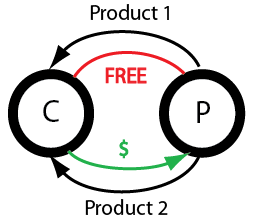
\includegraphics[scale=0.6]{figs/free1.png}}
    \caption{Cross subsidy between producer and customer, as employed by Gillette~\cite{chrisanderson2008}}
    \label{fig:gillette}
\end{figure}


One of the most important aspects of the freemium business model is that the few pay for the many. This is made possible through charging a small portion of the customer base, instead of charging the entire customer base with a smaller sum, which is visually represented by Figure~\ref{fig:freemium}. Additionally, the costs of providing a service to a non-paying customer must be kept to a minimum~\cite{chrisanderson2008feb}. There is however, a prerequisite for this to be work in practice, which is that it must be a digital market with inherent qualities such as very low to no distribution and production costs~\cite{chrisanderson2008}. Skype's former Vice President of Global Sales, Jonas Kjellberg, stated that a lot of Skype's early success could be attributed to pushing the product on a larger base of customers than what had previosly been done. This is in stark contrast to a more restrained approach normally taken during a customer acquisition phase~\cite{jonaskjellberg2014}. In terms of sales pipelines~\footnote{\textit{"the systematic application of scientific and mathematical principles to achieve the practical goals of a particular sales process"}~\cite{selden1996}}, a higher than normal amount of potential customers in, will eventually lead to a higher number of actual customers as a consequence.

\begin{figure}
    \centering
    \fbox{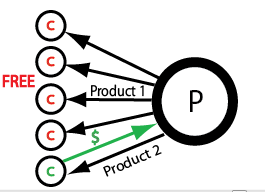
\includegraphics[scale=0.6]{figs/free3.png}}
    \caption{Visualisation of the interactions between producer and customer in the freemium model~\cite{chrisanderson2008}}
    \label{fig:freemium}
\end{figure}

Several definitions of freemium exists, but some of the most concrete has been stated by author, journalist and proponent of freemium Chris Anderson, who defines four different freemium models~\cite{chrisanderson2012}:

\begin{itemize}
    \item \textbf{Feature limited: }A basic version of the product exists alongside a more sophisticated, feature-rich paid version. Confirming to the try-before-you-buy mantra, customers are aware of the product they can potentially buy, which results in more loyal customers that are less price-sensitive. This is also the most suitable model for maximising reach among potential customers. In terms of downsides, there is a need to create two versions of what essentially are two very similar products. Retaining the number of free features is also detrimental to the success of this particular freemium model, as having too many features for free provides little incentive for the customers to pay for the premium version. Conversely, if too few features are included in the free version, users will lose interest in the product before they may purchase the premium version of the product.
    \item \textbf{Seat limited: }Allows for unlimited usage of the product, up to an arbitrary limit on the number of users. Should the number of users surpass this threshold, the product needs to be paid for. This is easy to implement and to understand, but it also runs the risk of cannibalising~\footnote{A market situation where a decrease in sales volume or market shares is a consequence of a new product being introduced, capturing a portion of the market~\cite{lifeofentrepeneur2015}} the lower ends of the market.
    \item \textbf{Time limited: }This model allows full usage of a product for a specified time period, after which the product needs to be paid for. This mitigates some of the threat posed by cannibalisation, and is relatively easy to implement. However, given that customers will not benefit from using the product after the specified time period unless they pay, induces a risk of customers not thoroughly committing to trying the product in the first place.
    \item \textbf{Customer type limited: }The product is offered freely to smaller and medium sized businesses, while larger enterprises and establishments have to pay. This provides some fairness, in that growing companies pay according to their ability, and enables growth among the smaller businesses and companies. However, arbitrarily defining the size, income, revenue and other factors of a business might be difficult. Where to draw the line between small enough to get it for free and large enough to pay might be complicated based on metrics and merits of a business alone. The \gls{b2b}-market has several actors that employs this particular freemium model, for instance Microsoft's BizSpark and Splunk. The former provides startups that have an income of less than 1 million USD per year with three years of software, services and support~\cite{microsoft2016}, and Splunk provides operational intelligence services at a discount for smaller IT environments~\cite{splunk2016}.
\end{itemize}


An important aspect concerning all free, digital products is how customers are able to access the service or product. Fred Wilson argues that customers should not have to download a digital product, which is why \gls{saas} can be a suitable platform for a freemium-based service~\cite{fredwilson20061}. Furthermore, the solution provided should be platform-agnostic, and barriers such as comprehensive registration should be avoided, as it might deter potential customers. This sentiment is paramount, since one of the main intentions of applying the freemium model is generating leads, thus increasing customer acquisition. Furthermore, creating demand for the premium features of a product or service, is almost equally important, since this is the main source of revenue for any business operating within the freemium model. In order to stimulate demand for premium features, these features should be clearly presented but not accessible to the users~\cite{bogdanpopescu2008}. Information on how to purchase premium features should also be clearly presented to the customers, because of the convenience this entails. Additionally, it is important to convey the value that premium features might add to the customer, and clearly stating what these do. 


When a customer base expands due to freemium being implemented, previous supporting capabilities provided by the business may no longer be sustainable. This will also hamper the ability to give customers adequate support, and may in turn generate bad-will sorrounding the product and brand name. To counteract this, a course of action that can be taken by a business in the freemium paradigm is offering substantial, thorough and clear instructions to customers about the product or service provided~\cite{brucehadley2003}. This alleviates some of the need for support in the first place, by enabling customers to more or less sustain their own usage of a product. Additionally, the creation of communities in the form of forums may be another way of solving the need for support. This also has the effect of having users engage amongst each other and may provide feedback to community managers representing the business. Furthermore, support and even counselling may be provided as a paid service to obtain another revenue stream, should the need present itself. 

\section{B2B \& B2C markets}
In a \gls{b2b} market the business transactions usually take place between two or more companies~\cite{jewels2001towards} seen in Figure~\ref{fig:b2b}, while in a \gls{b2c} market this transaction takes place between a business and a multitude of different consumers, as seen in Figure~\ref{fig:b2c}. These transactions often involve several people in the \gls{b2b} market, and is referred to as the decision making unit~\cite{paulhaguenickhaguematthewharrison}. These types of units are often dynamic and see frequent changes in memberships, and individual members may have opposing views or agendas. In the \gls{b2b} setting it is more reasonable to expect actors that are rational, while in the \gls{b2c} setting this cannot always be expected. Regular consumers are often more concerned with what they \textit{want}, while their business counterparts are often more concerned about what they \textit{need}. In terms of products and services offered in the various markets, complex products are more prevailing in the business market, often requiring a particular set of skills to use and operate. Another requirement often found in business markets is interoperability between products, where new acquisitions often have to be integrated with existing products and technical solutions in order to harness the value generated. Consumers might be concerned with the aesthetics of a product and hold that aspect in high regard, while businesses might value performance, security and longevity higher than aesthetics. 
\begin{figure}[H]
    \centering
    \fbox{\includegraphics[scale=0.3]{figs/b2b.png}}
    \caption{B2B interactions between the producer on the left and the purchasing entity consisting of several people on the right}
    \label{fig:b2b}
\end{figure}
Concerning sales volume, the number of units sold per customer in a \gls{b2b} market is often exceedingly larger than in a \gls{b2c} market, given that consumers are often limited by financial and volume-related aspects in purchasing products, while businesses have less restrictions on both of these aspects. As with niche markets, the Pareto (also known as the 80:20) rule applies to business markets as well, meaning that 80\% of the revenue is obtained from 20\% of the users. It can be reasonably predicted how much of a product a consumer will consume over a time period, but this is hardly feasible in a \gls{b2b} market: In a \gls{b2b} market, the difference in how much a business spends on a product or service will likely vary greatly compared to a consumer-based market. Conclusively, it can be stated that a business market contains few customers with greatly varying purchasing volumes, while a consumer market the purchasing volumes remains the same but the amount of customers may vary greatly.
\begin{figure}[H]
    \centering
    \fbox{\includegraphics[scale=0.3]{figs/b2c.png}}
    \caption{B2C interactions between the producer on the left and several, independent purchasing units on the right}
    \label{fig:b2c}
\end{figure}

\newpage
Business markets have a more uniform behaviour among its procurers and a smaller customer base overall than consumer markets. Thus, the different business market segments can be described in the following way:
\begin{itemize}
    \item \textbf{Service-oriented: }Primarily high requirements for quality and reliability, with delivery and after-sales also being of great importance. This category often pertains to businesses that belong in time-critical markets, with high sales volumes and establishments of any size.
    \item \textbf{Quality-oriented: }Most concerned about acquiring the objectively best product available, with a high willingness to pay. Medium to large sized companies working to high margins can be placed in this category.
    \item \textbf{Partnership-oriented: }Companies fitting into this category tends to be large and working to rather high margins, valuing trust and reliability. Businesses in this segment often see the service or product as a strategic partnership with another business, and the segment often concern key accounts.
    \item \textbf{Price-oriented: }The most transactional-centric segment, mainly interested in doing business avoiding as much superfluous activities as possible. Size-wise, often smaller companies working to low margins fall into this category, with the product or service being of low or little strategic significance.
\end{itemize}


Customer relationships tend to be more intimate in a \gls{b2b} setting, as it is arguably easier to maintain relationships with a lower number of customers. In contrast, a consumer market will often contain more customers overall, thus making a direct, bi-lateral relationship impossible on a larger scale. Business markets often tend to have a greater need for post-sales support than a consumer market. An example of this is printers: In a consumer setting there may be a handful of people using one printer from time to time, while a printer may be used extensively and by several people day in and day out in an office setting, which in turn creates a greater need for service being performed. Furthermore, losing a customer in a \gls{b2b} setting may have devastating consequences given the smaller customer base, making reliable customers and partnerships very desirable assets to businesses. The need to follow trends is much greater in a \gls{b2c} setting, making innovation less needed in a \gls{b2b} setting, consequently enabling businesses to follow trends rather than create them. As a consequence, businesses in a \gls{b2b} market are able to be risk-averse in their decision-making and generally experience less risk in their endeavours. A summary of the different characteristics of \gls{b2b} and \gls{b2c} marketing can be seen in Table~\ref{b2bb2c}.


\begin{table}[]
\centering
\caption{Important characteristics of B2B \& B2C marketing~\cite{teleopti2016}}
\label{b2bb2c}
\resizebox{\textwidth}{!}{%
\begin{tabular}{|l|l|l|}
\hline
\textbf{Characteristic}                                                                        & \textbf{B2C}                                                                                     & \textbf{B2B}                                                                                                      \\ \hline
Number and type of customers                                                                   & Many, small                                                                                      & Few, large                                                                                                        \\ \hline
Purchase orientation                                                                           & Individual or family needs                                                                       & Organisational and individual needs                                                                               \\ \hline
Nature of purchasing process:                                                                  & Simple, single-step                                                                              & Complex, multi-step                                                                                               \\ \hline
\begin{tabular}[c]{@{}l@{}}Number of people involved \\ in the purchasing process\end{tabular} & Small                                                                                            & Large                                                                                                             \\ \hline
Decision time                                                                                  & Short                                                                                            & Long                                                                                                              \\ \hline
Size of purchase:                                                                              & Small quantities and values                                                                      & Large quantities and/or values                                                                                    \\ \hline
Consequence of poor purchase                                                                   & Limited                                                                                          & Potentially critical                                                                                              \\ \hline
Nature of products and services                                                                & Standard range of products                                                                       & Customised packages                                                                                               \\ \hline
Pricing methods                                                                                & List prices                                                                                      & \begin{tabular}[c]{@{}l@{}}Quantity discounts, competitive bidding\\ and negotiation\end{tabular}                 \\ \hline
Distribution channel configuration                                                             & Complex and long                                                                                 & Simple and short                                                                                                  \\ \hline
Communication focus                                                                            & Psychological benefits                                                                           & Economic/utilitarian benefits                                                                                     \\ \hline
Primary communication mode                                                                     & Non-personal: Advertising                                                                        & \begin{tabular}[c]{@{}l@{}}Personal: Direct marketing and\\ personal sales\end{tabular}                           \\ \hline
Supplier switching costs                                                                       & Limited                                                                                          & Large                                                                                                             \\ \hline
Nature of relationships                                                                        & \begin{tabular}[c]{@{}l@{}}Low or moderate importance, \\ value chain relationships\end{tabular} & \begin{tabular}[c]{@{}l@{}}Close, strategic, interdependencies, \\ complex networks of relationships\end{tabular} \\ \hline
\end{tabular}%
}
\end{table}

\section{The case of B2B\&C}
\gls{b2bc} is a relatively new term, and is in many ways similar to \gls{b2b}, so much that it can be stated that it is an extension of \gls{b2b}. The main difference lies in who the value proposition is intended for: In \gls{b2bc} the value proposition is addressed to a business from another business, but the inherent value of the proposition is meant for a business' clients or consumers~\cite{Muzellec2015139}. This implicates that the service provided is not directly intended for the business, but rather for the procuring business' clients. Furthermore, the business on the receiving end in the \gls{b2bc} market can be seen as a supplier in the context of value chains, as opposed to the consumant role in the \gls{b2b} scenario. Co-creation may also be established between businesses in the context of value creation, and even the formation of key partnerships is not uncommon. One way to describe this interaction can be seen in Figure~\ref{fig:b2bc}.

\begin{figure}[H]
    \centering
    \fbox{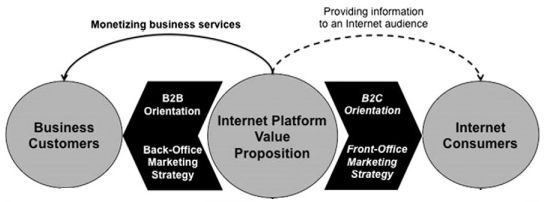
\includegraphics[width=\textwidth]{figs/b2bc.PNG}}
    \caption{B2B\&C interactions showing how value propositions are delivered~\cite{Muzellec2015139}}
    \label{fig:b2bc}
\end{figure}

To exemplify the notion of \gls{b2bc}: MazeMap provides a service to NTNU, but it's not the establishment itself (the business) that uses the service, but rather NTNU's clients which in this case pertains to students, staff and visitors. It is important to make the distinction that value is not only generated for a business' clients in this scenario, but can also greatly benefit the business in a reciprocal manner. The customer segment that is hospitals may be able to greatly benefit from this effect. By providing patients with information before they ever visit a hospital regarding where to park and where an appointment is to take place, can reduce stress among patients as well as saving costs related to missed or delayed appointments. In the case of Great Britain's \gls{nhs}, it was discovered that missed appointments accounted for annual costs of 800 million GBP~\cite{lucyjohnston2012}. This cost may be lowered by providing patients an \gls{ims}, and if 0,1\% more patients were able to attend their appointments on time, it would induce cost benefits~\cite{mazemaphospitals2015}.


\section{Preliminary work}
In the autumn of 2015, the author wrote a report that had a similar goal as this thesis, namely investigating if freemium had the potential to be a viable business model in a \gls{b2bc} market, and if it could accelerate customer acquisition. The main research done in this report was a survey that targeted more customer segments than this thesis, but done at a national level as opposed to an international level. The results from this report is used sparingly throughout this thesis, as the report struggled with obtaining a significant sample size for its survey. There are however parts where respondents of the survey gave more expanded answers compared to the survey in this thesis, and as such these results have been presented where appropriate. 

\chapter{Chapter 3 - Methodology}
This chapter introduces the reader to the the methodology of the research, investigative work, the subjects under scrutiny and how these leads to the results of this thesis.

\section{International Potential for Free Indoor Mapping Services Survey}
In order to get relevant information regarding the international market for free \glspl{ims}, and to obtain empirical evidence, a survey was conducted. The survey was done at an international level where respondents were asked to reply to a survey estimated to take between six and eight minutes. The main factor in choosing which \glspl{hei} to contact was the size of the institution, as these might have a larger and inherent need and demand for an \gls{ims}. 


The different institutions were contacted exclusively via email, with email and name of institution bein kept in a spreadsheet to avoid double-contacting people and institutions, while enabling the respective contacts of the survey to be re-contacted. Respondents were also welcome to answer the survey in other ways than Google Forms, but no responsents opted for this. Initially, only the absolute highest ranking official of any given institution was contacted, but consequently the invitation letter was altered slightly, to state that any person with relevant experience may answer the survey. The scope was then widened to include anyone from building- and facilites management, property management, information services management and a larger than initially group of senior officials. Media and communications departments were also contacted, as the invitation letter pleaded recipients to forward the letter to whom it might concern. To follow up non-respondents, each respondent was asked to state their email address and affiliation to avoid being contacted after completing the survey. A new list of non-responders was formed throughout the survey period, and sendouts were performed periodically. Furthermore, they were informed that the survey data was to be handled confidentially, and as such every email address from the survey has purposely been redacted in this thesis. The results can be found as a spreadsheet attachment. The first round of send-outs were conducted in March 2016, and the survey was concluded late June the same year. 

\subsection{Purpose of the Survey}
The primary goal of the survey was to assess and evaluate if customers in the \gls{b2bc}-market would be interested in a free \gls{ims}. The secondary goal of the survey was to assess the potential customer's willingness to pay for additional services, as this is crucial for the freemium model to be profitable. Additionally, respondents were asked whether or not an \gls{ims} was desirable in the first place. Lastly, a question was raised regarding the potential concerns in the event of a procurement, concerning demand, price and security concerns.

\subsection{Response Rate, Difficulties and Risks}
The main concern when formulating and conducting the survey at an international level, is in many cases the response rate. Given the importance of the empirical data from the survey, this was a concern from the beginning. 
\newline
\\
The invitation letter was aptly changed to accommodate for any shortcomings the plan for sending out emails had, to increase the number of respondents. Through an iterative process, the invitation letter was changed so that it was made clear that it was possible to answer the survey in a different way than through Google Forms i.e. via telephone or video conference, but none of the respondents opted for this option. Given the low response rate from the initial sendout, telephone calls where considered as means of getting in contact with the correct personnel, but this proved to be time consuming and to little use. During the time of a telephone call, the author would manage to get around ten more contacts through email leading to the abandonment of this method of reaching out. From initially only contacting between one and three individuals from an institution, this number was greatly increased through looking up email addresses from the websites of the respective institutions. This tactic increased the response rate from 5\% to nearly 20\%.  The length of the survey was engineered to be short, as leaders and other senior personnel often have a busy schedule. Additionally, the questions in the survey required little to no knowledge of any technical aspects regarding an indoor mapping solution. This was done in order to appeal to as broad an audience as possible. In total 198 institutions were contacted with 39 answers submitted. A total of 5517 emails were sent, making the average number of emails sent to each institution around 28. 
\newline
\\
During the first phase of the send-out a script handling sending emails spreadsheet was used. As described above, the spreadsheet contained a column with the numerous email addresses, while another column contained the invitation letter. The last two columns contained information whether the institution had already given an answer or didn't want to be involved with the survey, and the last column contained the name of the institution in order to have a better overview. The scripting language itself resembles JavaScript, and runs remotely on Google's servers~\cite{google2016} offering its user seamless integration across the various applications and services provided by Google. The source code of the script was inspired by online tutorials, and was customised for the purpose of sending emails using the information in the spreadsheet. The source code of the script can be seen in Listing~\ref{lst:email}. It should be noted that this way of sending survey invitations was abandoned at a later stage due to inherent limitations in Google's Gmail platform: A limit of 100 recipients per day was simply not enough when the total emails that was due for sending was over 5000. This resulted in abandonment of the script, in favor of using blind copies when sending the huge volume of emails. \gls{ntnu}'s Microsoft Office365 Mail was used instead, as it imposed fewer limitations in number of emails allowed to send during a 24-hour period.


The survey itself was conceived and presented in Google Forms, an easy and widespread method not only for making surveys, but also handling replies in spreadsheet form. The invitation letter contained a short URL of a link to the survey. Appendix B shows the survey as presented to the respondents, and Figure~\ref{fig:contactsheet} shows how respondents were being tracked.


\begin{figure}
    \centering
    \fbox{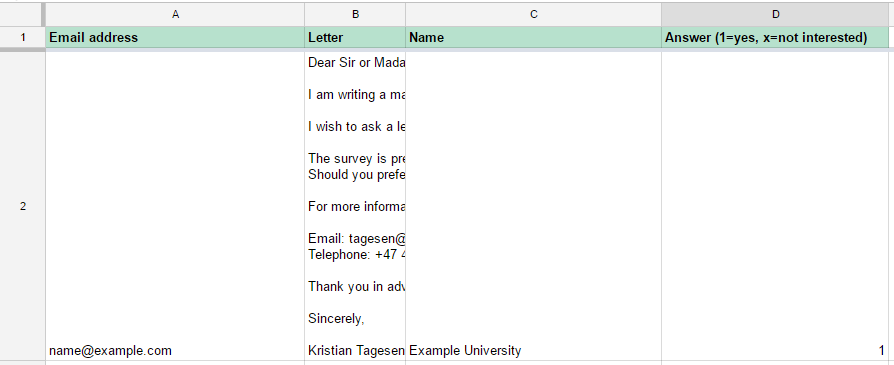
\includegraphics[width=\textwidth]{figs/contactsheet.PNG}}
    \caption{Spreadsheet used to keep track of potential respondents}
    \label{fig:contactsheet}
\end{figure}

\lstdefinelanguage{JavaScript}{
  keywords={break, case, catch, continue, debugger, default, delete, do, else, false, finally, for, function, if, in, instanceof, new, null, return, switch, this, throw, true, try, typeof, var, void, while, with},
  morecomment=[l]{//},
  morecomment=[s]{/*}{*/},
  morestring=[b]',
  morestring=[b]",
  ndkeywords={class, export, boolean, throw, implements, import, this},
  keywordstyle=\color{blue}\bfseries,
  ndkeywordstyle=\color{darkgray}\bfseries,
  identifierstyle=\color{black},
  commentstyle=\color{purple}\ttfamily,
  stringstyle=\color{red}\ttfamily,
  sensitive=true
}

\lstset{
   language=JavaScript,
   extendedchars=true,
   basicstyle=\footnotesize\ttfamily,
   showstringspaces=false,
   showspaces=false,
   numbers=left,
   numberstyle=\footnotesize,
   numbersep=9pt,
   tabsize=2,
   breaklines=true,
   showtabs=false,
   captionpos=b
}

\medskip
\begin{lstlisting}[caption=Email Sendout Script,label={lst:email}]
function sendEmails() {
  var sheet = SpreadsheetApp.getActiveSheet();
  var startRow = 2;  // First mail to send
  var numRows = 73;   // Number of emails to send
  // Fetch the range of cells included in this script
  var dataRange = sheet.getRange(startRow, 1, numRows, 2);
  // Fetch values for each row in the Range.
  var data = dataRange.getValues();
  for (i in data) {
    var row = data[i];
    var emailAddress = row[0];  // First column
    var message = row[1];       // Second column
    var subject = "Market potential for free indoor mapping services - MSc Survey";
    GmailApp.sendEmail(emailAddress, subject, message, {from: 'tagesen@stud.ntnu.no', name: 'Kristian Tagesen'});
  }
}
\end{lstlisting}


\section{Business Model Canvas}
%Skrive hvordan forløpet går gjennom de ulike delene av BMC
This section introduces the reader to the framework that is Business Model Canvas, used to describe the proposed business model in REF(CHAPTER XX). This particular framework has its merits in that it is used to invent, challenge and describe a business model \cite{strategyzer2016}. Further advantages include that it strips away any superfluous elements, improving its readability and enables users and business owners to focus on the most vital elements of a business model. It is also immensely flexible, as changes can be readily made without changing everything thanks to its modular design \cite{osterwalder2013business}. 
\newline
\\
\begin{table}[H]
\centering
\caption{Building blocks of the Business Model Canvas}
\label{tab:canvas}
\begin{tabular}{|l|l|}
\hline
\textbf{Product}                                    & Value proposition     \\ \hline
\multirow{3}{*}{\textbf{Customer interface}}        & Customer segments     \\ \cline{2-2} 
                                                    & Relationship          \\ \cline{2-2} 
                                                    & Distribution channels \\ \hline
\multirow{2}{*}{\textbf{Financial aspects}}         & Cost structure        \\ \cline{2-2} 
                                                    & Revenue stream        \\ \hline
\multirow{3}{*}{\textbf{Infrastructure management}} & Key partnerships      \\ \cline{2-2} 
                                                    & Key activities        \\ \cline{2-2} 
                                                    & Key resources         \\ \hline
\end{tabular}
\end{table}

The framework consists of nine building blocks with varying degrees of importance, but an important relationship between them. When all building blocks are determined, they make up the total strategy of how a business would operate, make money and if desired, capture market shares. Table~\ref{tab:canvas} shows the different building blocks by their respective categories, and Figure~\ref{fig:businessmodelcanvas} shows the empty template for setting up the business model. The business model canvas is described here, as it will serve as a template for the proposal of the business model. Below follows a step-by-step description of the respective building blocks.


\subsection{Customer segments}
This building block consists of the different customer segments a company wishes to concentrate on and reach out to. A market may be single or multi-sided, containing at a minimum a segment per market side. Media companies, credit card companies and to some extent social networking sites among others fall into a multi-sided market category. It is important to note that when offering a value proposition to a market, market size is an important factor, as smaller, niche markets may be a viable market segment as opposed to a bigger market. Finally, diversified products offered through the value proposition may be used to reach smaller subsets of the market.
\subsection{Value proposition}
The value proposition is the building block that describes how a company is different from other competing companies. It details how a company's products or services can create value for their respective customer segments, where values may be qualitative or quantitative. Several means of creating value among customers  includes lower pricing (price-sensitive segments), design (aesthetically appealing products), status (well-known brands), customisation (tailor-made services or products) and performance-driven products. Additionally, introducing a brand new disruptive technology i.e. cell-phones may benefit a business' customer segment, even though it may initially be viewed as unnecessary. Offering consultancy services can also be a value proposition in itself, for instance IT-consultancy services. Concretely, in the framework one wishes to map a value proposition to a particular customer segment, in order to identify the needs of this particular segment.
\subsection{Distribution channels}
Distribution channels concerns how a value proposition is delivered to a customer segment. A channel serves multiple purposes, with the most important being raising awareness around the products or services a company is offering and aiding customers in understanding the value propositions. It also serves a perhaps equally important function in allowing for products or services to be purchased. Furthermore, the channels can be broken into different phases, depending on what phase a product is in. These include:

\begin{itemize}
    \item \textbf{Awareness}: Raising awareness among customers.
    \item \textbf{Evaluation}: How customers are able to evaluate the value proposition.
    \item \textbf{Purchase}: How products are purchasable from the customer's point of view.
    \item \textbf{Delivery}: How a value proposition is delivered to a customer.
    \item \textbf{After sales}: How on-going customer support is handled post-purchase.
\end{itemize}
Along with the next block, Customer relationships, the channels block forms how a business interfaces with their customers. 

\subsection{Customer relationships}
The different types of relationships a business establishes with their respective customer segments are detailed in the customer relationships block. From a business' perspective, having good customer relationships may entail several benefits in increasing their sales volume, gaining new customers and keeping their existing customers from leaving. The perhaps simplest relationship between a business and a customer lies in personal assistance, where actual, dedicated personnel from the business side is serving any customer need from any part of the sales cycle. In a \gls{b2b} market one may have one dedicated person or team per customer, while in a \gls{b2c} market this might not be manageable and call centres or e-mail respondents serves the purpose better. On the flipside, having customers manage themselves entirely either through robust online self-services or inter-customer relationships is also an option depending on the product or service provided. Lastly, co-creation where companies and customers share responsibility for the product is a modern take on a customer relationship, seen in social networks and user-creation oriented services i.e. YouTube.

\subsection{Revenue streams}
How much cash-flow each customer segment generates constitutes the revenue stream building block. It is essential for the profitability of a product or service, with revenue streams being either a one-time fee or recurring payments. Several ways to generate revenue streams include:

\begin{itemize}
    \item \textbf{Subscription fees: }By selling a service, a business may charge its customers of that service for any given time period. 
    \item \textbf{Licensing: }In companies where some form of intellectual property is made, it is possible to generate revenue by the sales or lending of these properties.
    \item \textbf{Advertising: }This type of revenue stream is generated from advertising a product or service on the behalf of some other business entity.
    \item \textbf{Brokerage fees: }By providing services between two parties and taking a fee for the transactions that take place.
    \item \textbf{Asset sale: }Selling the rights to one instance of a product falls into this category, and is the most traditional way of exchanging goods.
\end{itemize}

At this point of setting up the model, the customer segments are linked to its respective value propositions. Each of these should at this point be linked with a revenue stream.

\subsection{Key activities}
The key activities are the detrimental matters that a business needs to attend in order to deliver its value propositions. Together with key resources they are vital in creating and offering the value proposition to the customers, earning revenues and keeping customers satisfied. Consultant and service-oriented businesses often revolve around problem solving as a key activity, helping others with new and existing problems. For manufacturing companies and businesses, proposing, making and delivering products is a key activity, while software and banking service businesses may have a robust platform they offer their customers. In the case of the latter, the platform itself is the main component of their key activities. Lastly, it is important to connect the key activities to the value propositions, as the key activities are the main drivers of the value propositions.

\subsection{Key resources}
The key resources in this framework is absolutely vital for businesses in order to provide and create value propositions for its customers. Together with the key activities, they enable the generation of revenues, maintaining customer relationships and reach markets. Several types of key resources include:  physical (buildings, manufacturing plants), human (consultancy and r\&d services), financial (gaining and edge on competitors by lowering the price point) and intellectual (intellectual properties, brands etc.). The goal 
of the key resources is for the business to surpass competitors on key areas of the key resources.

\subsection{Key partnerships}
This building block concerns the partnerships, suppliers and other third party entities needed to make the business model work. The partnerships can vary in nature, where competitors and non-competitors can forge alliances or creating joint ventures. Any non-in-house solutions have to be supplied by third parties be it manufacturing parts or personnel. Motivations for creating partnerships include optimising the allocation of resources, reducing risk and to cut down on activities not vital in delivering a final product or service. As such, key partnerships can be linked with activities that aren't necessarily key to drive a business' value proposition. 

\subsection{Cost structure}
Different cost structures include fixed costs, variable costs, economies of scope and economies of scale. Fixed costs are volume-independent, and is usually examples of employee salary, rental costs and other facilities. Variable costs are volume-sensitive, while economies of scale concerns the costs changing as a result of a change in the scale of operation. Economies of scope on the other hand benefits businesses that diversify the number of different products or services offered, and is volume-insensitive in this regard. Different cost-structures exist in cost-driven and value-driven models. The former focuses on minimising the costs, and the latter model fits companies that less concerned with price and focuses more on value creation.
Lastly, it is important to note the relationship between cost structures and key activities, as the key activities drive a business' cost structures. 

\begin{figure}[]
\centering
\includegraphics[width=10cm]{figs/busmodcanvas.png}
\caption{Business Model Canvas template. \textcopyright businessmodelgeneration.com}
\label{fig:businessmodelcanvas}
\end{figure}

\chapter{B2B Case Studies}
In this chapter, \gls{b2b} solutions that have previously been under scrutiny will be discussed. Firstly, two case studies "Freemium for Large Enterprises" by Jepson, Lundin (2011)~\cite{jepson2009freemium} and "B2B Sales and Marketing Plan For Limecraft", Lamminpää, Kalle (2014)~\cite{lamminpaa2014b2b} will be reviewed, then two proven and successful freemium-based businesses will be under scrutiny. This is done in order to propose a better business model in Chapter 6
.
\section{"Freemium for Large Enterprises" by Jepson, Lundin (2011)}
Freemium for Large Enterprises by Jepson, Lundin (2011) concerns the viability of freemium as a business model in expensive and advanced solutions in an enterprise market, and revolves around the Swedish software development company Teleopti.

\subsection{About Teleopti}
Teleopti is a world leading company in delivering software solutions for strategic workforce management (WFM) and telecom expense management (TEM). Their product offering is twofold, consisting of Teleopti CCC for WFM and Teleopti Pro for TEM. As far as sales channels are concerned, their products are purchasable directly from them, as well as from partner resellers throughout the world. A Workforce Management (WFM) product makes sure that appropriately skilled personnel is placed at the correct place at an correct time. WFM contains six core parts: forecasting, staffing, scheduling, operating, analysing and reporting, with the forecasting module being a main proponent given that its function is to try to predict staffing needs at various times. These parts can be seen in Figure~\ref{fig:wfm}. Teleopti CCC is the focal point in this study, as the thesis by Jepson \& Lundin pertains to this particular product. The WFM service provided by Teleopti aims to to optimize the performance of contact centers, back offices, branches and retail stores, by managing staffing needs according to the workload. The solution is also agent-centric meaning that the workforce members are able to access the service through smartphones or other mobile platforms, while being able to manually control scheduling, monitor staffing needs in real-time and self-administer working shifts.  
\begin{figure}[H]
    \centering
    \fbox{\includegraphics[scale=0.6]{figs/WFM.png}}
    \caption{The circular WFM process}
    \label{fig:wfm}
\end{figure}
Teleopti's CCC product has a modular design and features a basic package, with several additional modules being available for purchase. The basic package contains the modules Forecast, People, Shifts, Schedules, Intraday, MyTime and Reports. The Forecasts module predicts workload, Shifts optimises the schedule from the predicted workload generated by the Forecasts module, People manages staff, Intraday monitors workload in real-time and takes action should workload exceed a certain threshold. Reports generates logs, enabling an evaluation of operations and MyTime is used by the staff to view reports and schedules. Optional modules include Performance Manager for a more advanced Reports module, Real Time Adherence for monitoring staff in real-time, Payroll Integration for salary management and Employee Self Service, an employee tool for messaging and shift planning. The main building blocks of Teleopti CCC can be seen in Figure~\ref{fig:teleopticcc}.

\begin{figure}[H]
    \centering
    \fbox{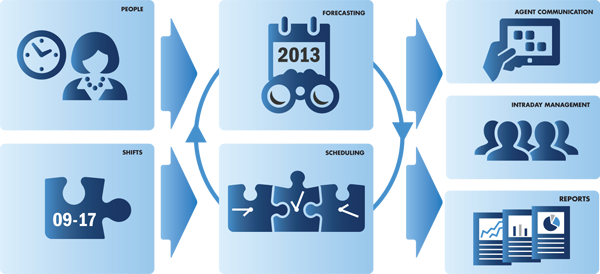
\includegraphics[scale=0.5]{figs/teleopticcc.png}}
    \caption{Teleopti CCC's core functionality represented by its modules~\cite{teleopti2016}}
    \label{fig:teleopticcc}
\end{figure}

\subsection{Results}
Teleopti already has an established and premium product in Teleopti CCC, and with it being modular in design, a module could be selected as being the focal point for generating leads in transitioning to a freemium model. Reasons for the selection of only one free module included modularity, creating demand for premium parts of the product and less adjustments needing to be made. Their recommendation fell on the Forecasts module as its features was possible to be used in isolation. Furthermore, this module was seen as a high-intensity feature of the product, as well as being a cornerstone in any WFM solution. It was further speculated that this module itself would generate the most demand for additional modules. A potential downside in choosing this model was the requirement of data from external sources.


Several points were made to generate demand for the premium parts of the product, and as such it was suggested that additional paid features were left in, but greyed out leaving some of the features visible but not usable. However, technical limitations made this impossible and these additional modules were instead featured on the Teleopti Help webpage. In an effort to create as low entry barriers as possible, it was the decided that the best course of action was to simply require registration from users of the product. An emphasis was put on leads generation as a main proponent of a freemium model, and as such contact information from the free users was deemed necessary in order to raise demand for the premium parts of the product. Manual authorisation of new customers of the free part was suggested, as having documentation and instruction only available to authorised users would make it harder for competitors to gain a competitive advantage on Teleopti as well as bringing a feeling of exclusiveness to its users.
\newpage
It was pointed out that thorough documentation needed to be in place in a freemium product, to make sure new users adopt to the product and to minimise support costs. Comprehensive documentation for different levels of user proficiency was therefore suggested, to minimise support costs for the Teleopti support team. Having a larger user base as a result of freemium would also lead to more bug discoveries and fixes, easily remedied by patching the product for premium and free users alike. This can be seen as a positive externality as a result of an increased customer base using a freemium business model. 


Marketing Teleopti's brand and product were viewed as key success factors. The two main goals of launching a freemium product were to increase leads generation (thusly accelerating customer acquisition) and to raise awareness around Teleopti's brand. It was pointed out that Teleopti wished to state clear intentions when gaining new customers, in that their goal was to eventually sell their premium product, as having a hidden agenda may prove to have adverse effects in a \gls{b2b} setting. It was deemed important that in all communications had a clear message of what they were selling, how much it cost and that the free product is a part of a larger software package. Given that \gls{b2b} marketing differs from \gls{b2c} marketing, it was suggested that the channels used for marketing include the Internet, newsletters, business partners and press releases. Given Teleopti's intentions of eventually selling their premium product, it was deemed necessary to rigorously follow up on free customers. This was realised by sending out a questionnaire to and telemarketing the customers of the free product. 
\newpage
In conclusion, several success factors were listed as being detrimental for a freemium model in a \gls{b2b} market:
\begin{itemize}
    \item \textbf{First-to-market: }More attention for the target market through PR and word-of-mouth. 
    \item \textbf{Adequate marketing communication: }Make sure there is no gap between the target market of the free and premium product, due to the lead-generating aspect of freemium. Use appropriate marketing channels. Stimulate partners to market the free product, and clearly convey the type of product offered.
    \item \textbf{Stimulating demand for the premium product: }Make users aware that premium features or products exists, aswell as the brand of the premium product while following up on potential leads among the free users. 
    \item \textbf{User-friendly processes and product: }Have a robust and informative website with a simple and straightforward registration and installation process. Easy to follow and comprehensive documentation to reduce support costs, with support being free of charge.
    \item \textbf{Self-serviced customer services: }No internal resources needed for using the free product among customers, and keeping the free and premium equivalents close in function to avoid high maintenance costs. 
\end{itemize}

\section{"B2B Sales and Marketing Plan For Limecraft" by Lamminpää, Kalle (2014)}
Lamminpää's thesis revolves around the Belgian start-up company Limecraft, in the business of media production. Founded in 2010, it delivers a product called Flow; a cloud-based software allowing media producers to share and collaborate their productions with each other~\cite{lamminpaa2014b2b}. This is a new way of moving footage between different personnel as opposed to the traditional way of transferring physical media physically. 


According to Lamminpää, Limecraft surveyed the large market that is the media industry, and estimated that around 2.5 million professionals worked in this field worldwide. In its infancy, Limecraft marketed their Flow product in the \gls{sme} market as a freemium-based service. Onwards they discovered new markets in universities that often handle huge amounts of video in digital lectures etc. As in Freemium for Large Enterprises by Jepson, Lundin (2011), a large emphasis is put on leads generation. In Limecraft's case this was done at a large scale at the  Marché International des Programmes de Télévision (MIPTV) event in France where media professionals meet annually. Other trade fairs are also cited as being valuable venues for leads generation, as well as having a orderly website with clearly stated goals. 


Limecraft's freemium model was also described in a different manner than Teleopti's: A free product was offered upon registration with 2.5GB of media storage, with this being expandable by inviting new users to the product or by upgrading to a premium payment model. However, issues arose when this particular model allowed for perpetual expansion of storage space and was consequently changed to a hard limit in volume of 5GB and only lasting three months. This is radically different from the freemium model proposed by Jepson \& Lundin (2011), and thusly the model offered by Limecraft can be viewed as being a trial version as opposed to freemium. A problem that followed was that the user-base didn't churn towards the premium product as expected. 


To remedy this several proposals were made by the Lamminpää: A larger social media presence, namely at Twitter, LinkedIn, through blogs and Slideshare, in order to be more visible on Google's search engine. Limecraft's sales cycle was reported at being around six months, making each customer more valuable. Freemium can possibly shorten the sales cycle~\cite{davidskokN/A}, but this is not mentioned by Kalle in this case. In conclusion, Lamminpää notes that a more aggressive marketing strategy should be employed, by empowering the social media presence of Limecraft, in addition to focusing on attending more trade conventions for leads generation. 


This particular case was included to demonstrate a company that has somewhat failed at employing the freemium model successfully, having reverted to a more traditional business model. This may be attributed to several factors including an inappropriate market for freemium products and Limecraft's reluctance in developing their product into the business paradigm that is freemium. 
\newpage
\section{Successful B2B Freemium Ventures}
This section contains the author's reviews of two services within the \gls{b2b} market that has successfully implemented a freemium model: Box and Splunk. These will be introduced in addition to having their potential success factors discussed.
\subsection{Box}
\subsubsection{About}
Box was founded in 2005 by Aaron Levie and Dylan Smith, offering online file sharing and content management services for businesses. The free part of Box is limited to personal accounts for one users, with limits imposed on both storage and maximum file size. The premium part allows for enterprise and business accounts with potentially limitless storage options. Several users per account is also allowed, with better collaboration, administration and security features~\cite{freemium.orgN/A}. In 2010 they reported having a userbase of 10 million users divided amongst 120,000 businesses, with a free-to-premium churning rate of 8\%. Additionally, Box claims that 82\% of the largest companies in the world uses Box.
\subsubsection{Success factors}
Some of Box's success can be attributed to the ideas emerging from Box's leaders: They have stated that technical solutions are first and foremost used by its actual users, not management. This is reflected in their business model which only offers free Box accounts to non-enterprise entities, in the hope that that these users will act as proponents of Box's products in their respective businesses. Another important philosophy stated by Levin is the importance of keeping customers in a \gls{saas}-setting happy~\cite{tientzuozuora2014}\cite{youtube2011}. They believe happy customers are more willing to pay as long as a good product is in place to begin with, a prerequisite of the freemium business model. The use of the freemium model (albeit in an indirect way in a \gls{b2b} setting), allows for penetration in markets previously being thought of as unreachable. Furthermore it is pointed out that in a freemium paradigm, non-paying customers are not lost to competitors.


As a company that delivers \gls{saas} services, revenues has to be viewed in a different manner than traditional means, where \gls{arr} is a better metric. It is self-explanatory that in the long-term this can be more profitable, and this is shown in the Gross Recurring Margin for Box estimated at 79\% in 2014~\cite{tientzuozuora2014}. This shows that their costs are acceptable, and furthermore, their Recurring Revenue Margin (\gls{arr} minus sales, R\&D and G\&A costs) grew from 8\% in April of 2013 to 20\% in January of 2014. These facts combine may indicate that Box is an expanding and profitable business. Lastly, Box also has an \gls{api}, enabling users of Box to customise and integrate Box into existing systems, apps and services. Box also allows external innovation through their provided \gls{api}, making it possible for developers to make apps in the Box ecosystem and monetise these apps. 

\subsection{Splunk}
\begin{figure}[H]
    \centering
    \fbox{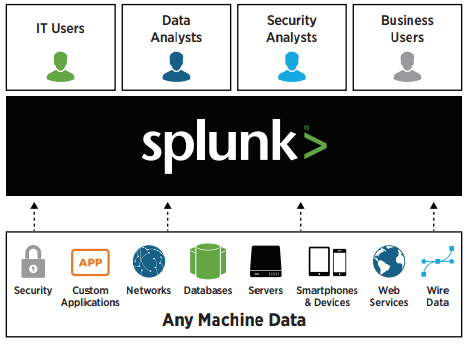
\includegraphics[scale=0.8]{figs/splunk.PNG}}
    \caption{Splunk's Enterprise product~\cite{splunkinc20162}}
    \label{fig:splunk}
\end{figure}
\subsubsection{About}
Splunk was founded in 2003 by Michael Baum, Erik Swan and Rob Das, and is a software company producing software for analysing, monitoring and searching big data~\cite{derrickharris2010}. Splunk offers their software either as a platform or \gls{saas}, and features these either as an Enterprise package or a Light package with the latter being aimed at smaller IT environments. The difference between these two lies in their respective premium packages: Light has a limit on daily data volume and maximum users, while Enterprise does not have this limitation. The rest of the differences are smaller in magnitude, but Enterprise customers can also access the \glspl{api} and enjoy more rigorous support. The \gls{saas} versions operate on a free trial basis with a limit on 5GB of cloud storage per day, while the platform versions have a limit of 500MB of indexed data per day. After 30 days of usage, the users of the platform-version may continue with a free license or upgrade to a premium version. Splunk's revenues were estimated to have increased by 50\% from 2015 to 2016, expecting annual revenues around 850 million USD. They have more than 10 000 customers across 100 countries and 1700 employees.

\subsubsection{Success factors}
Initially, only the platform version of Splunk was offered but they later expanded to a subscription-based \gls{saas} offering, representing 37\% of revenues. Focus was also shifted towards enterprise customers as opposed to \gls{smb} customers, and they report that up to 70\% of customers convert their free licenses to premium ones, utilising the additional features the premium model offers~\cite{philiplay2014}. Much of Splunk's success also comes from providing a mission-crucial service in security and IT services, and focuses more and more on sales and customer support given its growth. The rich information and real-time analysis provided by Splunk enables its customers to avoid security threats, monitor customer preferences, launch new products faster and saving money in the process. One of Splunk's main value propositions is to provide its customers with usable, valuable and accessible big data, eliminating any inherent inefficiencies among customers. 
\chapter{The International Market Survey - Results}
\renewcommand{\arraystretch}{1.5}
This chapter is intended to present the results from the International Survey to the reader, with the questions and responses being presented and discussed here. In total, 193 different \glspl{hei} were contacted and 39 respondents submitted answers. This yields a response rate of over 20\%. 
\section{Respondents}
Replies from different countries are represented in Table~\ref{contactedcountries}, and geographically in Figure~\ref{fig:worldmap}. The color code used in this figure represents which countries that had \glspl{hei} contacted, where red indicates no reply from any \gls{hei} in that country, and green indicating one or more replies from a \gls{hei} in that country. The "Other" category that contains four possible answers, were respondents who failed to denote what institution they were representing, and no indication of who they were representing were given whatsoever. After the initial sendout, the chosen \glspl{hei} contacted were adjusted in order to obtain more data from the survey. This was done by contacting more \glspl{hei} from countries with a good response rate. Countries with English as a first language are also more represented, and as such there may exist a correlation between this and the response rate from these countries. In general more European countries replied to the survey, and apart from any possible language barriers, the websites of \glspl{hei} from western countries were generally more open and informative, making it easier to find the correct person to contact. 


Several respondents indicated that they were some sort of leading figure (as per request in the invitation letter); building- and facilities managers, senior leadership and general operations managers. In one case, a European university opted to have three different personnel respond to the survey. These results are also included, due to the varying nature and different point of views these persons may have. Given the anonymity of the survey, no names of personnel or institutions will be given in this thesis, since none of the contacted \glspl{hei} agreed to disclose such information. However, the country of origin and the respondent's position is revealed where possible. 


\begin{table}[H]
\centering
\caption{Number of contacted \glspl{hei}, replies and response rate by country}
\label{contactedcountries}
\begin{tabular}{|l|l|l|l|}
\hline
\textbf{Country} & \textbf{Contacted} & \textbf{Replies} & \textbf{Response rate} \\ \hline
Austria          & 3                  & 1                & 33.3\%                 \\ \hline
Denmark          & 3                  & 3                & 100.0\%                \\ \hline
Finland          & 5                  & 3                & 60.0\%                 \\ \hline
Germany          & 12                 & 3                & 25.0\%                 \\ \hline
Indonesia        & 3                  & 1                & 33.3\%                 \\ \hline
Ireland          & 4                  & 3                & 75.0\%                 \\ \hline
Italy            & 3                  & 1                & 33.3\%                 \\ \hline
Japan            & 3                  & 1                & 33.3\%                 \\ \hline
South Africa     & 3                  & 2                & 66.7\%                 \\ \hline
Switzerland      & 5                  & 3                & 60.0\%                 \\ \hline
Thailand         & 3                  & 1                & 33.3\%                 \\ \hline
The Netherlands  & 14                 & 5                & 35.7\%                 \\ \hline
United Kingdom   & 17                 & 5                & 29.4\%                 \\ \hline
USA              & 65                 & 3                & 4.6\%                  \\ \hline
Other            & 50                 & 4                & 8.0\%                  \\ \hline
\textbf{Total}   & \textbf{193}       & \textbf{39}      & \textbf{20.2\%}        \\ \hline
\end{tabular}
\end{table}

\newpage
\begin{figure}[]
    \centering
    \fbox{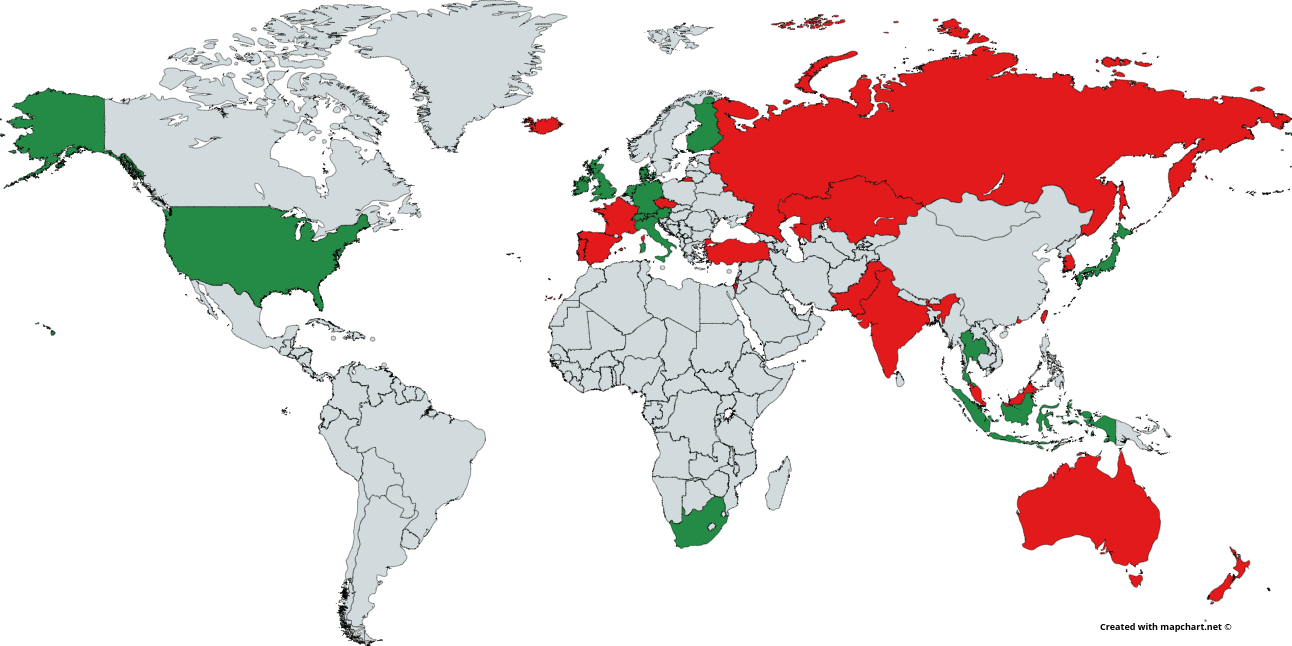
\includegraphics[scale=0.25]{figs/worldmap.png}}
    \caption{A geographical representation of countries in which \glspl{hei} were contacted. Red denotes no replies from that country, while green indicates one or more answer being submitted}
    \label{fig:worldmap}
\end{figure}

\section{Introductory questions - Question Group 1}
Table~\ref{surveyquestions} shows all questions asked in the survey according to their respective group of questions. Questions have been grouped in a manner that will present the survey results in a clear way for the reader. The first group of questions are introductory questions, concerning the respondent's current indoor mapping situation. After respondents stated their affiliation, the question "Are you currently using an indoor mapping service?" (Q1) was asked, with results shown in Figure~\ref{fig:q1}. The rationale behind this question, was to see if it was possible to churn existing \gls{ims} users to a freemium-based \gls{ims}. Conversely, respondents replying "no" are also interesting subjects for the surveyor. These represent potential first-time procurers of an \glspl{ims}, and together with those who replied "Yes" in Q2 they make up potential customers. The majority of respondents (64,1\%) had no \gls{ims} in place, while 35,9\% stated that they have an \gls{ims} in place. 

\begin{figure}[H]
    \centering
    \fbox{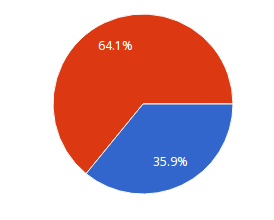
\includegraphics{figs/q1.png}}
    \caption{Q1: "Are you currently using an indoor mapping service?". Blue indicates "Yes" and red indicates "No"}
    \label{fig:q1}
\end{figure}


Based on the response given in Q1 respondents were either forwarded to Q2 or Q3. Respondents stating that they already employed an \gls{ims} were forwarded to Q3, while those without an \gls{ims} were routed to Q2. Q2 asked respondents without an \gls{ims} if they were willing to consider using an \gls{ims}. This was posed in order to gauge and measure the respondent's willingness for procurement and interest in an indoor mapping system, with results shown in Figure~\ref{fig:q2}. A total of 25 respondents replied to this question, due to this question being irrellevant for those previously stating that they already have an indoor mapping system. A majority of 68\% replied that they were willing to consider using an \gls{ims}, while 32\% stated that an indoor mapping system was not something they would consider using. To follow up on the latter group, a qualitative question in Q2.2 was asked, where respondents were asked to state the reason as to why they would not consider such a service. Question 2.2 was not mandatory, but 3 respondents chose to reply. However, these replies contributing little to the results of this thesis.


\begin{figure}[H]
    \centering
    \fbox{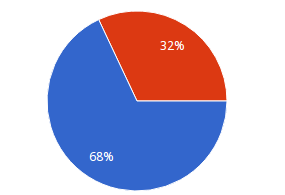
\includegraphics{figs/q2.png}}
    \caption{Q2: "Are you willing to consider using an indoor mapping service?". Blue indicates "Yes" and red indicates "No"}
    \label{fig:q2}
\end{figure}


\begin{table}[]
\centering
\caption{Questions asked in the International Market Survey}
\label{surveyquestions}
\resizebox{\textwidth}{!}{%
\begin{tabular}{|c|c|c|l|}
\hline
\textbf{Keyword} & \textbf{} & \multicolumn{1}{l|}{\textbf{\begin{tabular}[c]{@{}l@{}}Question\\ Group\end{tabular}}} & \textbf{Question phrasing}                                                                                                                                                                                                                                             \\ \hline
Q1               &           & 1                                                                                      & Are you currently using an indoor mapping service?                                                                                                                                                                                                                     \\ \hline
                 & Q2.1        & 1                                                                                      & Are you willing to consider using an indoor mapping service?                                                                                                                                                                                                           \\ \hline
                 & Q2.2      & 1                                                                                      & If no, please state the reason as to why this is not desired                                                                                                                                                                                                           \\ \hline
Q3               &           & 2                                                                                      & \begin{tabular}[c]{@{}l@{}}Given an indoor mapping service that will entail\\ several benefits for your institution, \\ please rate the initial interest in such a service\end{tabular}                                                                                \\ \hline
Q4               &           & 2                                                                                      & \begin{tabular}[c]{@{}l@{}}How much of an concern would price be in procuring \\ an indoor mapping service?\end{tabular}                                                                                                                                               \\ \hline
Q5               &           & 3                                                                                      & \begin{tabular}[c]{@{}l@{}}Please rank the following services in terms of willingness to pay: \\ "Navigation \& indoor pathfinding", "Timetable integration", \\ "Integration with SMS, apps, IT-infrastructure etc." \\ and "Automatic updating of maps"\end{tabular} \\ \hline
Q6               &           & 4                                                                                      & \begin{tabular}[c]{@{}l@{}}Which factors would be of concern when procuring\\ an indoor mapping service?\end{tabular}                                                                                                                                                  \\ \hline
\end{tabular}%
}
\end{table}

\section{Measuring Interest - Question Group 2}
This section contains questions engineered to measure the interest for \glspl{ims} in a quantitative manner. The first question Q3 was formulated as follows: "Given an indoor mapping service that will entail several benefits for your institution, please rate the initial interest in such a service". Additionally, respondents were presented with examples of how an \gls{ims} could benefit their institution~\footnote{Improve visitor experience by showing them where to go, how to get there and even where to park. Improve employee efficiency by showing new personnel i.e. cleaning personnel around campus without the need for a dedicated guide. Improve the experience for students by alleviating stress and uncertainty by showing students and staff alike to the correct location in time for class. Additionally, an indoor mapping enables service personnel to readily locate the place of interest as opposed to decoding a textual description.}. Possible answers were presented on a Likert scale with 1 denoting "Not interested at all" and 5 denoting "Highly interested".


Figure~\ref{fig:q3} shows the results from Q3. Looking at the statistics from Table~\ref{q3q4stats} a mean of 3,872 and the most common answer being "Interested (4)", it can be argued that an initial interest for \glspl{ims} exists. This further reinforced by the fact that 64,1\% showed initial interest in such a service in Q1. These results can be said to conclusively point towards a definite interest in \glspl{ims} among the respondents. 32\% were initially not willing to consider using an \gls{ims} (Q2), but after being presented with the potential benefits of an \gls{ims}, this number was lowered to 15,4\%. This can be viewed as a positive trend, but it can also indicate that the market surveyed in this case is not aware of the possible positive benefits an \gls{ims} entails.


\begin{figure}
    \centering
    \fbox{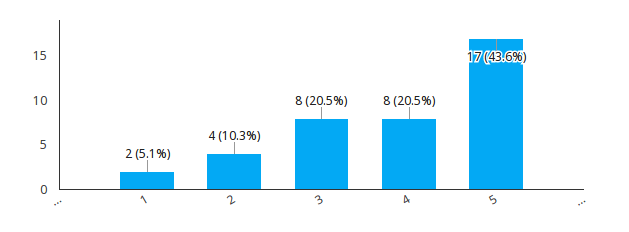
\includegraphics[width=\textwidth]{figs/q3.png}}
    \caption{Results of Q3: "Given an indoor mapping service that will entail several benefits for your institution, please rate the initial interest in such a service". Vertical axis denotes number of responses.}
    \label{fig:q3}
\end{figure}



Similar to Q3, Q4 was posed as a quantitative question and asked respondents "how much of an concern price would be in procuring an indoor mapping service". This question aimed to measure the viability of freemium in the \gls{b2bc} paradigm. A low concern for price might indicate that freemium itself is not a main proponent in accelerating customer acquisition, and conversely a high concern for price would indicate a certain viability for freemium among price-sensitive customers. Compared to Q3, this question garnered even more positive results: A mean of 4,026 and a median of 4 indicates a trend that the respondents were price-sensitive. Further cementing this notion is the fact that 76,9\% of respondents viewed price as a somewhat high to a high concern. In a non-freemium business paradigm these results would potentially be negative indicators, as price-sensitive customers could potentially lead to a enlonged sales pipeline. However, in the freemium paradigm these are excellent results, since price seems to be a major factor in the potential procurement of an \gls{ims}. The results from this question can be seen in Figure~\ref{fig:q4}



\begin{table}[]
\centering
\caption{Statistics: Question Group 2}
\label{q3q4stats}
\resizebox{\textwidth}{!}{%
\begin{tabular}{|l|l|l|}
\hline
\textbf{Parameter} & \textbf{Q3: Interest} & \textbf{Q4: Concerning price} \\ \hline
Sample size        & 39                    & 39                            \\ \hline
Mean               & 3,872                 & 4,026                         \\ \hline
Median             & 4                     & 4                             \\ \hline
Mode               & Interested (4)        & Somewhat High Concern (4)     \\ \hline
\end{tabular}%
}
\end{table}


\begin{figure}
    \centering
    \fbox{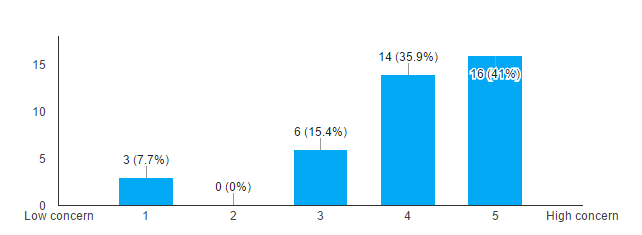
\includegraphics[width=\textwidth]{figs/q4.PNG}}
    \caption{Results of Q4: "How much of an concern would price be in procuring an indoor mapping service?" Vertical axis denotes number of responses.}
    \label{fig:q4}
\end{figure}

\section{Interest for Premium, Value-Adding Services - Group 3}
This group of questions contains one question, divided into 4 subquestions. Thusly, the different questions will hereby be reffered to as Q5.1, Q5.2, Q5.3 and Q5.4. For this group of questions, respondents were asked to rank four different \gls{ims}-related services in terms of willingness to pay, where 1 indicated a low willingness to pay, and 5 indicating a high willingness to pay. Under each service, the respondents were informed about why these features might be beneficial to their institution, akin to Q3. The statistics of these questions can be seen in Table~\ref{q5stats}. In the freemium paradigm with the few paying for the many, it is important that premium features are implemented for the sake of profitability. However, freemium in a \gls{b2b} or \gls{b2bc} market is more than often used as a potent leads-generator~\cite{jepson2009freemium}. Due to this, the willingness to pay for the premium features are not detrimental for successfully applying freemium in this case, thus making any negative feedback on premium, value-adding services not necessarily speak against freemium. Lastly, it should be noted that any initial disinterest from respondents are further compounded in this group of questions, and the numbers should be viewed accordingly.

\begin{table}[]
\centering
\caption{Statistics: Question Group 3}
\label{q5stats}
\resizebox{\textwidth}{!}{%
\begin{tabular}{|l|l|l|l|l|}
\hline
\textbf{Parameter}      & \textbf{Q5.1} & \textbf{Q5.2} & \textbf{Q5.3} & \textbf{Q5.4} \\ \hline
Sample size             & 39            & 39            & 39            & 39            \\ \hline
Mean                    & 2.59          & 2.538         & 2.769         & 2.872         \\ \hline
Median                  & 3             & 3             & 3             & 3             \\ \hline
Mode                    & Neutral (3)   & Neutral (3)   & Neutral (3)   & Neutral (3)   \\ \hline
Willing to pay (4 \& 5) & 24.4\%        & 31,7\%        & 31,7\%        & 36.6\%        \\ \hline
\end{tabular}%
}
\end{table}


For this Q5.1 the respondents were given the following potentially beneficial features of indoor navigation and pathfinding:

\begin{displayquote}
\textit{"While not a necessary component of an indoor mapping service, navigation and indoor path finding can help users find their desired location. A plethora of technologies exist for this purpose using existing Wi-Fi infrastructure, Bluetooth, beacons, smartphone sensors, magnetic positioning etc."}
\end{displayquote}

Figure~\ref{fig:q51} shows results from Q5.1. The statistics show a mean of 2,59 and a median of 3 making the mode "Neutral (3)". These numbers do not indicate a strong willingness or lack thereof of this particular feature, and represents the third most popular premium service. The numbers are however, slightly on the positive side of the scale with a non-negative median, however there were equally many neutral as there were those with low willingness to pay for this type of service. \gls{mm} has stated that their primary focus is making the indoor maps themselves, and as much as 80\% of its users do not use any form of indoor navigation (Jelle, personal communication 17.09.2015). This fact is to some extent reflected in these results. The respondents were however not informed that an \gls{ims} such as \gls{mm} has a partner in Cisco that enables the usage of existing Wi-Fi infrastructure for positioning and navigation. Given that indoor navigation techniques are in its infancy, it can perhaps be expected to see a rise in the technologies applied in this field in the future. 

\begin{figure}[H]
    \centering
    \fbox{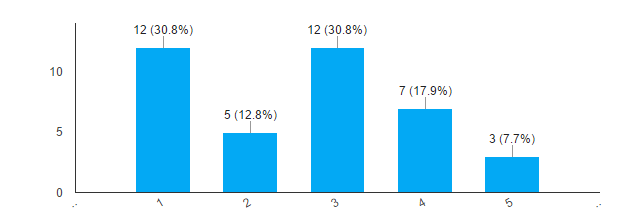
\includegraphics[width=\textwidth]{figs/q51.PNG}}
    \caption{Results of Q5.1: "Navigation and indoor pathfinding". Vertical axis denotes number of responses.}
    \label{fig:q51}
\end{figure}

Q5.2 asked the users to rate their willingness to pay for timetable integration. Respondents were presented with the following potential benefits:

\begin{displayquote}
\textit{" "Where", "how" and "when" are commonly asked questions when an appointment is due or a meeting is taking place. Timetable integration aims to answer the two former questions by providing an indoor map and which path to take to get there."}
\end{displayquote}

With a mean of 2,538 and a median of 3, this was the least popular of the presented value-adding services. Figure~\ref{fig:q52} shows the results being quite even on all but one of the possible answers, likely indicating a divided set of responders. As with Q5.1, these numbers to not indicate any trends of strong or weak desires towards this type of service, but it is important to emphasize that some respondents were unfamiliar with \glspl{ims} in general, or had no desire to acquire one. In hindsight, the author could have provided respondents of the survey with visual rather than textual examples of the value-adding, premium services to give respondents a better overview of the implications and usefulness of these services. 


\begin{figure}[H]
    \centering
    \fbox{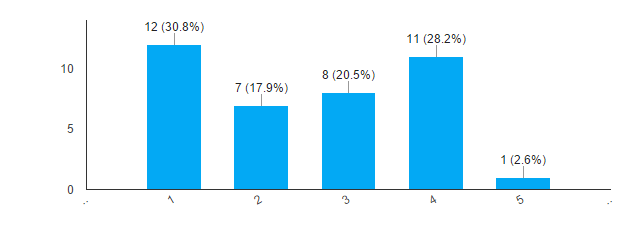
\includegraphics[width=\textwidth]{figs/q52.PNG}}
    \caption{Results of Q5.2: "Timetable integration". Vertical axis denotes number of responses.}
    \label{fig:q52}
\end{figure}


The next question in the group concerned the integration of an \gls{ims} into SMS, applications, IT-infrastructure etc. Potential benefits were proclaimed as follows:

\begin{displayquote}
\textit{"An API that integrates indoor maps with the existing services mentioned above, aims to enable seamlessly integrating indoor maps into already existing systems and services without the need to manually do so for every service."}
\end{displayquote}

The results of this question can be seen in Figure~\ref{fig:q53}, with a mean of 2.769 and median of 3 making it the second most popular service presented, with 61,6\% of replies being Neutral (3) and above. As stated previously, it must be stressed that it might be hard to visualise how these premium features work in a concrete scenario. If potential \gls{ims} buyers are largely unaware of the benefits, it can make this particular service a hard sell. Furthermore, integrating an \gls{ims} into existing infrastructure might represent a security risk for the procuring part. This pertains to any potential security holes an \gls{ims} might have, and if such holes are present, malicious users are potentially able to gather sensitive data such as passwords and user-names. Therefore, it was expected that this question would score low, but the results shows it being on par with the others.  

\begin{figure}[H]
    \centering
    \fbox{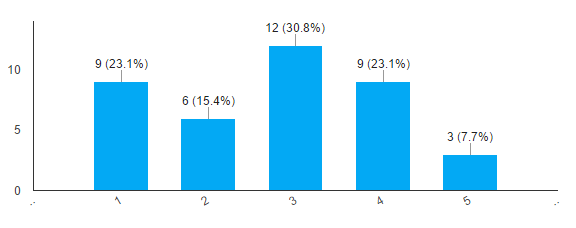
\includegraphics[width=\textwidth]{figs/q53.PNG}}
    \caption{Results of Q5.3: "Integration with SMS, apps, IT-infrastructure etc.
". Vertical axis denotes number of responses.}
    \label{fig:q53}
\end{figure}

The last question in the group, Q5.4, asked respondents to rate a service that automatically kept maps up to date. Respondents were presented with the following key features of this particular value-adding service:

\begin{displayquote}
\textit{"Larger establishments tend to change over time, and often see around 10\% of buildings change anually\footnote{Jelle, personal communication, 25.09.2015}. Manually updating indoor maps can therefore be a tedious and time-consuming activity."}
\end{displayquote}

Figure~\ref{fig:q54} shows results from Q5.4, with a mean of 2.872 and a median of 3 (Neutral). For respondents unaccustomed to \glspl{ims}, this question would perhaps be the hardest to answer, since it directly revolves around an \gls{ims}. As stated in earlier, \glspl{hei} may see over 10\% of its structures change during the course of a year. This is possibly reflected in the statistics, as they show this feature being the most popular of the four. It also had the highest number of interested respondents at 35,9\%. It can be speculated that the \glspl{hei} contacted in relation to the survey were aware that updating floor-plans could be quite an undertaking, and an \gls{ims} with this feature would be well received. 


\begin{figure}[H]
    \centering
    \fbox{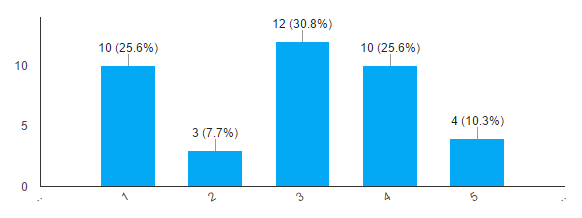
\includegraphics[width=\textwidth]{figs/q54.PNG}}
    \caption{Results of Q5.4: "Automatic updating of maps". Vertical axis denotes number of responses.}
    \label{fig:q54}
\end{figure}

\newpage

\section{Potential Procurement Concerns - Question Group 4}
The final group of questions asked concerned potential aversions that the \glspl{hei} contacted might have. At the end of the survey, respondents were welcome to freely add anything concerning the survey, the free model or \glspl{ims}, but few chose to do this. The rationale behind having this question group was to map the potential hinderances in procurement of an \gls{ims}. The question asked in this section consisted of checkboxes where respondents were free to mark as many options as desired, and an overview of the replies is shown in Table~\ref{q6}. Respondents were free to interpret "Security Concerns" in their own way. However, it was the author's intention to gauge if the respondent owning the rights to the indoor maps themselves was a concern or not.


\begin{table}[H]
\centering
\caption{Overview of data from Q6}
\label{q6}
\begin{tabular}{l|l|l|l|l|}
\cline{2-5}
                                           & \textbf{Price} & \textbf{Demand} & \textbf{Security Concerns} & \textbf{Other} \\ \hline
\multicolumn{1}{|l|}{\textbf{Sample size}} & 39             & 39              & 39                         & 39             \\ \hline
\multicolumn{1}{|l|}{\textbf{Quantity}}    & 33             & 19              & 23                         & 8              \\ \hline
\multicolumn{1}{|l|}{\textbf{Percentage}}  & 84.6\%         & 48.7\%          & 59.0\%                     & 20.5\%         \\ \hline
\end{tabular}
\end{table}

Q6, the final question of the survey prompted the respondents with the following: "Which factors would be of concern when procuring an indoor mapping service?" Four different factors were presented, and respondents were allowed to choose all four should they so desire, with the different options being "Price", "Demand", "Security concerns" and "Other". The "Other"-option allowed respondents to shortly describe a potential concern not applicable to the above. The results of this question can be seen in Figure~\ref{fig:q6}, and some of the "other"-factors were suggested as follows:
\begin{itemize}
    \item \textit{"Accuracy and legibility"}
    \item \textit{"Maintenance"}
    \item \textit{"Integration with reservation system"}
    \item \textit{"Ease of use, accessibility and [the] ability to administer system locally"}
    \item \textit{"Quality of the service such as usability and features"}
    \item \textit{"Content"}
    \item \textit{"Campus user experience"}
\end{itemize}

Some of these factors pertains to the actual usefulness of the service itself, while some concern the user experience. Although \gls{b2b} and \gls{b2bc} markets have many similarities, this can be said to be a difference in this case: As the purchasing business in a \gls{b2bc} scenario governs the the service provided to its clients, quality, ease of use and usefulness are factors that must not be overlooked in the case for \glspl{hei}.



\begin{figure}[H]
    \centering
    \fbox{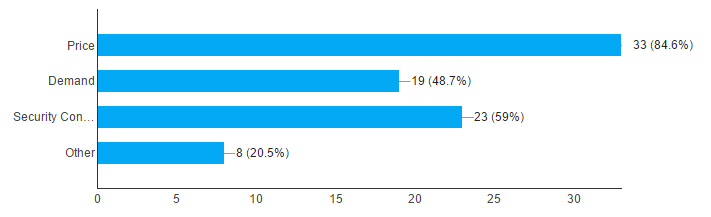
\includegraphics[width=\textwidth]{figs/q6.PNG}}
    \caption{Results of Q6: "Which factors would be of concern when procuring an indoor mapping service?". Horizontal axis represents number of responses. Option 3 not wholly visible: "Security Concerns".}
    \label{fig:q6}
\end{figure}

The most chosen factor was "Price" at 84,6\%, followed by "Security Concerns" at 59\%, "Demand" at 48,7\% and "Other" at 20,5\%. Given that Q4 showed that most of the respondents were concerned about price, this trend is further confirmed in this question. For unaware readers, it might be hard to grasp that citing "Price" is not a given factor in the procurement of a service or product. It is interesting however, due to the market segment discussed in this thesis (\glspl{hei}) might not be as price sensitive as other parts of the market. Many of these are publicly owned, and as such long-running costs may be more of a concern. In the case of potential public procurements, countries in the EU and countries like Norway have laws regarding public procurement practices and regulation~\cite{europeancommision}\cite{procurement}. In the preliminary research paper, the author reviewed a similar research question constrained to the Norwegian market. In terms of Norway's public procurement laws, it is stated that if any public entity wishes to purchase a certain service, that type of service has to be announced publically. Offering bids from potential outreachers is usually the norm, and after a certain amount of time an eventual procurement can take place. A similar survey was offered in this paper where one respondent from a Norwegian Hospital stated~\cite{kristiantagesen2015}:
\begin{displayquote}
\textit{"We have to deal with the rulings of public procurement, and it would be the total cost that is the underlying factor. The content of the "basic" package is detrimental to a potential procurement, as it may trigger further needs for more services. If a(n) [indoor mapping] system can satisfy the demands and rules of a public procurement, then [a freemium-based \gls{ims}] is of interest".}
\end{displayquote}
In terms of the viability of freemium in this scenario, this can be viewed positively and negatively: The positive aspect of this is that potential leads and prospects in an organization that is in a procurement phase, might convince senior management personnel more easily, to obtain a service that will cost nothing initially. On the other hand, long-term and total costs may be more concerning for potential procurers than a service or product being free initially. As stated by the above respondent, the contents of the non-premium parts were detrimental, and may trigger the need for purchasing premium parts of the product or service.
\chapter{Proposal of Business Model}
This chapter will present the reader with the freemium-based business model proposal for MazeMap. It will be proposed based on findings and results from other parts of this thesis, particularly from Chapter 4 \& 5. The Business Model Canvas described in Appendix C will be used as a fundamental framework to describe and realise the model.


\section{The Freemium Indoor Map Service Business Model}
\subsection{Customer Segments}
While this thesis has primarily been focused on one customer segment, namely \glspl{hei}, an \gls{ims} provider such as \gls{mm} may focus on additional customer segments: Hospitals, venues and shopping malls (along with \glspl{hei}) constitutes \gls{mm}'s self-described customer base~\cite{mazemap}. Furthermore, more specific and niche markets can be described in cruise ships, sporting arenas (football stadiums, car-racing arenas etc.), airports and museums. The actual procurers of MazeMap are senior personnel within any aforementioned institution or organisation, that govern the procurement activities. Focusing on the customer segment presented in this thesis, a divide can be said to exist between publicly owned \glspl{hei} and privately owned \glspl{hei}. These may have different emphasis on price in long or short terms. Public institutions may be more concerned with total costs and the quality, ease-of-use and usefulness of a service, while private institutions may be more sensitive to price in order to satisfy shareholders by keeping procurement costs down. All \glspl{hei} contacted were selected on a criterion of being of a certain size in terms of staff and enrolment. In the survey, Q6 indicated that "demand" was a possible deterrent from an \gls{ims}, and this option was more than often selected by \glspl{hei} smaller in size compared to the rest of the respondents. As such, this should be taken into account when targeting \glspl{hei} as a customer segment.

\newpage
From the customer's perspective, a low amount of financial means is needed in order to obtain \gls{mm}'s \gls{ims}. Having existing infrastructure such as Wi-Fi for implementing navigation features, might be seen as a requisite from the customer's perspective, should they desire navigational features. Given the characteristics of \gls{b2bc}, any procurers of an \gls{ims} should have an already established consumer base, with students and staff constituting \glspl{hei}' customer base. To sum up:


\begin{itemize}
    \item Procurers of MazeMap: Someone who governs procurement activities
    \item Freemium might be harder to implement due to regulatory affairs
    \item What needs to be in place customer side: Low amount of financial means, optionally Wi-Fi for navigation and an existing base of clients
\end{itemize}

\subsection{Value Propositions}
How a service generates value is instrumental in choosing target customer bases. \glspl{hei} are able to benefit from an \gls{ims} such as \gls{mm} for a plethora of reasons: As explored in International Business Potential for Analytics of Room Utilisation~\cite{karlbernhoffbinde2015}, by increasing room utilisation through analytics of how space is being utilised leads to several potential benefits: Increasing enrolment, reducing maintenance cost, alleviating environmental stress and reducing opportunity costs. \glspl{hei} experience an influx of new students and staff at the beginning of semesters, and an \gls{ims} can save both time and frustration among these in relation of finding their way around campus. Additionally, visitors are able to streamline their visiting experience by having an \gls{ims} provide parking instructions. Furthermore, \glspl{hei} are often the site of conferences consisting of first-time visitors who also can benefit greatly from finding out where to go and at what time, given \gls{mm}'s integrability with time-table and scheduling systems. Among both external and internal maintenance personnel, an \gls{ims} enable less time being spent on finding the correct place to be and lets personnel do their tasks more effectively, while greatly reducing the need for new staff to be shown around. 


With interactive maps allowing both customised and automatic generation of meta-data, an \gls{ims} can provide its users with fleet management. This is related to how users can find and locate equipment, both emergency-related equipment such as fire extinguishers and non-critical equipment such as printers. In this context, the emergence of the Internet of Things is also applicable, given that a lot of previously autonomous systems are now interconnected. An \gls{ims} enables tracking of these assets, and can satisfy the demand for making these things visible to its users.  Another important use-case is how a fire department can save time in critical moments by using an \gls{ims} to discover and locate fires or other accidents, as opposed to decoding messages from a fire alarm system. In the context of another customer segment not explicitly discussed here (hospitals), it is possible to save costs by reducing the number of missed appointments~\cite{mazemaphosp}, by employing an \gls{ims}. This can also be applied to \glspl{hei} albeit at possibly smaller cost savings, due to \glspl{hei} not being as appointment-based as hospitals.  


In terms of freemium, there are obvious cost savings for procurers of freemium-based \glspl{ims}. As the \gls{b2b} sales pipeline is longer than in a \gls{b2c} setting, a try-before-you-buy product may prevent compounded costs as a result of a long sales process. As was stated by the respondents of the survey, price presented an entry barrier to the potential purchase of an \gls{ims}, and there were some willingness to pay for some additional services. By taking this into account, this bodes well for implementing a freemium-based \gls{ims}. To summarise:

\begin{itemize}
    \item Digital interactive maps
    \item Optimise utilisation through analytics
    \item Directions for meeting-place and nearest parking for visitors
    \item Reducing uncertainty and stress for new students and staff
    \item Maintenance personnel: Professions that see frequent changes of staff and working locations. Indoor maps enable these to find their way quicker, saving personnel costs
    \item Fleet management, equipment tracking and the Internet of things
    \item Alarms shows up on maps rather than a code for a specific location. Can save time in emergency situations
    \item Reduce missed appointments
    \item Provide places of interests visually as opposed to textually
    \item For freemium: Cost savings by being free initially
    \item For freemium: Try before you buy, no big initial investment. Purchase according to need
    \item For freemium: Further value-adding services
\end{itemize}
\newpage
\subsection{Channels}
In order to be able to deliver its value propositions to the customer, a company delivering an \gls{ims} must use appropriate sales channels. Given that indoor maps is still a relatively new service, determining what channels to use can be difficult. It should be stressed that given the survey's respondents unfamiliarity with indoor maps, that such a service needs to emphasise its potential through value propositions, and bring awareness around them. Being an early mover proved to be important in the case of Teleopti discussed in Chapter 4, and given the fact that only 35\% of respondents already employed an \gls{ims}, further validates this notion. 


In terms of accelerating customer acquisition, the direct approach often taken in other \gls{b2b} scenarios may prove to be counter-productive for this purpose. First, the value proposals have to be brought forth to decision makers at an \gls{hei}. Then a top-down or a down-top recommendation may occur: If senior personnel take a liking to the service, their authority on the matter may influence its users (which are the consumers in the \gls{b2bc} setting) to start using a service. This is the top-down approach. The down-top approach occurs whenever demand for such a service starts with the consumers either through word-of-mouth or by users who have seen an \gls{ims} in action at another institution, similar to Box. This may in turn influence decision makers by wanting them to satisfy their respective consumers. As an \gls{ims} obtains more customers, the latter approach becomes more attractive, as its user base expands creating a demand that was scarce in the first place. The former approach can also greatly benefit from this through cross-references such as when success stories between \glspl{hei} are shared. This of course can also generate bad-will, should the service provided turn out to be lacking. During the initial roll-out phase of a freemium-based \gls{ims}, direct contact may be an important channel, however, as customer acquisition and lead generation become more important factors, direct contact becomes too time consuming and should be reserved customers who represent a larger business potential. As suggested by Lamminpää in Chapter 4, being visible at trade conventions may be a good tool for leads generation by direct contact. As opposed to the previously mentioned outreach-based direct contact, being visible at events hosted by organisations such as \gls{scup}, \gls{tefma}, \gls{cele} and \gls{appa}, may prove to be a more effective way of acquiring new customers from the \gls{hei} customer segment. Lastly, this channel type handles almost all of the product phases mentioned in Appendix C, barring after-sales.


MazeMap's webpage may also be used increasingly as a sales channel in the case of delivering a freemium-based service. As discussed in Chapter 4, entry barriers should be kept as low as possible. If the webpage is used as a sales channel it needs to provide adequate information regarding the value propositions offered to enable users to evaluate these propositions. Additionally, a service such as Google AdWords as employed by Limecraft, may also strengthen the webpage as a sales channel, by bringing awareness around the service provided. Given the \gls{saas}-nature of the product, the webpage can be used as a vessel to deliver the product to customers, and while users in the freemium paradigm do not purchase anything in the traditional sense of the word, the purchasing part could be handled by requiring users to register as the only barrier for using the service. To go with this, thorough and clear documentation should also be provided for these customers. Any premium parts of the service could be greyed out, but made readily purchasable depending on the service. 


Through \gls{mm}'s partnership with Cisco, the Cisco marketplace is another available sales channel~\cite{ciscomarket}. This platform provided by a well-known actor such as Cisco presents great publicity through the its brand, which provides services that are likely to meet any security concerns. Cisco is also a licensed, worldwide reseller, which may yield great value as a sales channel. Below is a summary of the various channels:


\begin{itemize}
    \item Direct approach
    \item Develop leads among potential customers
    \item Webpage
    \item Cisco marketplace
    \item For freemium: Hard to argue against initial high costs as with a non-freemium system
\end{itemize}

\subsection{Customer Relationships}
The need for establishing good and reasonable customer relationships is great, and in the case of freemium, generating leads is the most desirable outcome. These relationships changes as the product goes through different phases. Table~\ref{classiccr} shows a possible strategy for customer relationships under a non-freemium model, which focuses mostly on personal relationships. In a freemium model with a rapidly accelerated customer acquisition process, this can possibly lead to increased cost in staffing, sunk costs and costs resulting from failed sales. Therefore a more automated customer relationship model must be presented, seen in Table~\ref{relationshipstrat}. This attempts to combat the need for staffing dedicated to different parts of the sales cycle, by moving towards an autonomous, self-servicing system as the service matures. By providing rigorous documentation and self-help tools for the non-paying customers, as well as reaping potential benefits from communities around the product getting traction, this should be readily implemented. Lastly, as the service grows in users the number of bugs may increase, and as such, patches that are platform-wide and payment model-agnostic should be in place to maintain customer satisfaction.


\begin{table}[]
\centering
\caption{Customer relationships for different product phases, classic model~\cite{karlbernhoffbinde2015}}
\label{classiccr}
\begin{tabular}{|l|l|}
\hline
\textbf{Phase} & \textbf{Customer Relationship Strategy} \\ \hline
Pilot          & Co-creation, key partnerships           \\ \hline
Introduction   & Dedicated Personal Assistance           \\ \hline
Growth         & Personal Assistance                     \\ \hline
Maturity       & Communities                             \\ \hline
Decline        & Self Service                            \\ \hline
\end{tabular}
\end{table}


\begin{table}[]
\centering
\caption{Customer relationships for different product phases, freemium model}
\label{relationshipstrat}
\begin{tabular}{|l|l|}
\hline
\textbf{Phase} & \textbf{Customer Relationship Strategy}    \\ \hline
Pilot          & Dedicated personal assistance, co-creation \\ \hline
Introduction   & Self-service, personal assistance          \\ \hline
Growth         & Automated services                         \\ \hline
Maturity       & Communities                                \\ \hline
Decline        & Self-service                               \\ \hline
\end{tabular}
\end{table}

Emphasis should also be put on the creation of communities and cross-reference sales, hereunder inter-customer interactions. This to enable users to share knowledge and develop good usage practises, alleviating some of the need for customer service, should the service expand with the freemium model applied. The nature of the service does not induce competition among customers, and as such there is little to no point in not sharing the experiences of an \gls{ims}. On the contrary, the value and performance of the service may increase for all parties involved, which can only be viewed in a positive way. 


With freemium comes additional freedom in how a product is bundled. A solution like \gls{mm}'s can easily be modularised, with more full-fledged customer support, guidance or even \gls{crm} as premium features. By monetising this part of the service at a mature product stage, means that any early movers will not feel deterred from obtaining this type of service. Smaller and medium sized venues who may have less requirements from an \gls{ims} would ideally not need support if the self-support tools are sufficient in themselves, and larger institutions may be the target customer segment for more extensive and paid support features. Below is a summary of the proposed customer relationships:

\begin{itemize}
    \item As service matures, less active relationships, more automation
    \item Interactions between the businesses under the B2B\&C paradigm, sharing of experiences
    \item For freemium: Guidance as a paid service
\end{itemize}

\subsection{Revenue Streams}
Given that \glspl{ims} are still in its infancy product phase-wise, establishing that the services provided can be value-adding is important. Additionally, even though no monetary investment is needed upfront from the customer's perspective, the survey indicated that there are other factors such as demand and security concerns that may hinder the procurement of an \gls{ims}. It must therefore be communicated extensively that those factors should be of no concern by, for instance, pointing out the partnership with Cisco for security concerns and clearly communicating the value proposals in order to create demand. The future might bring additional need for services hitherto unknown, and these should be included as part of the \gls{mm} product range, to create a lock-in effect. 


In choosing which parts to be free and which ones that should be monetised, several considerations must be made: Create too few free modules and the service provided might be lacking for its purposes and create no demand. Creating too many free modules will risk cannibalisation the low end of the market~\cite{keller2011strategic} and generate little to no revenue. Considering these options, it might be better to initially offer too few modules as \gls{mm} already has an established customer base. While the survey showed that the lack of demand of an \gls{ims} is present, it could be risky to dedicate too much resources in offering non-paying customers modules or features should otherwise be monetised. 


Several parts of \gls{mm}'s product exists, which can be decomposed into different modules described in Table~\ref{modules}. For applying a successful freemium strategy, the choice of module(s) to include for free is crucial. The free parts should include the bare minimum for an \gls{ims}: An indoor map, basic map editor and an application to view the indoor map. Any additional services should be monetised. There are several ways to monetise the modules not included in the free package and as such two different payment models can be presented:


\begin{table}[]
\centering
\caption{Proposed modularisation of MazeMap}
\label{modules}
\resizebox{\textwidth}{!}{%
\begin{tabular}{|l|l|l|}
\hline
\textbf{Indoor maps}                             & \textbf{Integration} & \textbf{Navigation} \\ \hline
Map editor: basic                                & SMS notification     & Indoor positioning  \\ \hline
Map editor: advanced                             & Room reservation     & Indoor pathfinding  \\ \hline
Interactive maps (browser only)                  & Applications         &                     \\ \hline
Interactive maps (any platform)                  & IT-systems           &                     \\ \hline
Facility management (automatic updating of maps) & Timetables           &                     \\ \hline
Analytics                                        & API/SDK              &                     \\ \hline
Automatic updating of maps                       &                      &                     \\ \hline
\end{tabular}%
}
\end{table}

\subsection{Subscription}
As with Box (presented in Chapter 4) a subscription model for the premium, value-adding services may be implemented. For services such as analytics and automatic updating of maps and metadata a recurring payment model makes sense, given that they depend on several variables that may change customer-side. Other premium modules such as advanced map editors, platform independence and integration may not be as applicable to a subscription based payment model. However, there is nothing directly speaking against this way of monetising a service. Given that \gls{mm} delivers a \gls{saas}, operational costs must be taken into account, and subscription based features may cover these costs accordingly. After registering and uploading floor plans, users should be presented with a dashboard of the services available to them. The additional premium modules may be greyed out and activated when desired. This will then in turn induce either monthly or yearly recurring payments, depending on the type of service. Given that buildings change more slowly than points of interest, different rates of recurrent payments should be presented depending on the module. Additionally, usage quotas may be introduced. This works slightly different than the previously mentioned model; some modules are free to use and try out. The difference between the free and premium in this instance, is that free users are able to use premium features, but only up to a certain cap. This cap may let the premium features be time-limited or data-volume-limited, with restrictions removed upon setting up a payment plan.  

\subsection{One-time payments}
More in line with traditional, non-recurring payments, several of the modules fit better into this category, as opposed to the subscription model. Under this model customers would be presented with the premium modules greyed out, and pricing info on the respective models. Customers wanting to activate a particular module for their institution may do so after paying a one-time fee for said module. Under this model, the aforementioned time or data volume limitations on premium features may be imposed as an alternative way of trying out the various services. It should be noted that combining these two models is also a possibility, by having some modules appropriately subscription-based and some one-time-fee-based.


Free trials of the different premium modules can also be offered to be more in line with the try-before-you buy sentiment, central to the freemium business model. Additionally, some features can be free on rotation, for instance from one month to the next, which may increase the interest in some of the less popular features. This also opens up the possibility of evaluating the premium features available, by adjusting the price for less popular modules, while increasing price for the modules in demand. It is also possible to bundle some of the premium features, as a technique to reduce customer's ability to evaluate and reserve themselves at given price points. This provides a lock-in effect among customers, and may reduce the starting costs associated with enabling some of the premium services. To sum up:

\begin{itemize}
    \item Concept of freemium: The few pays for the many
    \item Subscription based premium modules
    \item One-time payment premium modules
    \item Bundling
\end{itemize}

\subsection{Key Activities}
Along with the key resources, the key activities form the way value propositions are delivered to the customers. Given the \gls{saas} nature of the product delivered, software development can be listed as one key activity, which relates to the ongoing development and maintenance of the key resource that is \gls{mm}'s platform. While operating within a freemium business model, a more secluded approach might be taken in terms of business development. Targeted marketing and sales should be reserved to larger customers, since one of the main goals of freemium is to accelerate customer acquisition. On that note, it is important for a supplier of an \gls{ims} not to completely forego this type of customer under the freemium paradigm, as that will leave the larger enterprise market largely untouched. When a customer has registered in order to use the free parts of the \gls{ims}, it is important to provide sufficient support and documentation, in order for customers to get up an running, thus retaining the customer base. Customers will quickly lose interest in a new type of service provided such as an \gls{ims}, if adequate introduction to the product is absent. As such, providing this can be seen as a key activity. 
\newpage

Roughly 80\% of \gls{mm}'s user-base don't use any form of positioning services, so customers wanting the indoor navigation and pathfinding modules may be directed towards the solution provided by \gls{mm}'s partner Cisco for implementation of the Wi-Fi based navigation feature. There are however, a plethora of emerging technologies that provide this, some with far greater accuracy than what is possible with Wi-Fi: iBeacons (\gls{ble}-based, signals between smartphone and beacon)~\cite{ibeacon2016}, IndoorAtlas' IPS system (geomagnetic indoor positioning, smartphone with magnetic sensors reacting to earth's magnetic fields)~\cite{indooratlas2016} and Sensor Fusion by indoo.rs (using a smartphone's built in sensors)~\cite{indoo.rs2016} to name a few. \gls{mm} has stated that supporting more positioning and navigation features will be made possible should there be a demand for them in the future (Jelle, personal communication 17.09.2015). Integrating maps into a customer's existing IT-systems and maintaining the map data and metadata can also be viewed as a key activity, providing a certain lock-in effect among customers. 


After purchases, emphasis should be put on maintaining the platform ensuring that a good and stable service is provided to the customers. The premium modules should act as means of revenue, and together with maintaining the platform it forms an important key activity, as it is vital for customer retention and may hamper the creation of communities. Enabling community creation post-sales should also be viewed as being paramount. This can be done through official forums, where users share both share knowledge and solves problems together, as may be necessary in the event that the customer base expands rapidly. Again, this to minimise supporting costs, however some customers with more advanced needs who operate on a larger scale may need dedicated personal assistance. In turn, this customer group is also expected to pay for more premium features, possibly covering the support cost margin.

\begin{itemize}
    \item For freemium: Providing adequate level of support, particularly during the implementation phase
    \item Key Account management and business development - large customers with many needs
    \item Indoor mapping constitutes roughly 80\% of usage
    \item Accommodating for indoor navigation and pathfinding via Cisco and other partners
    \item Integration of maps
    \item Reworking and updating map data and metadata
    \item Integration into booking systems
    \item Marketing, sales and customer support
    \item After purchase: Revenue through premium modules
    \item After purchase: Enabling community creation 
\end{itemize}

\subsection{Key Resources}
Since the method of delivery of \gls{mm} is \gls{saas}, several resources needs to be allocated in order to provide and create the services needed to fulfil the value propositions. \gls{mm}'s servers containing the service provided, is a hugely important asset in this case. Without these, the service would not be able to be offered as a \gls{saas}. Having a centralised, consolidated infrastructure enables faster bug-fixing, and will provide customers with an up-to-date version of the services at all times. Regarding freemium, the most important aspect of the key resources is the engine that converts floor plans to interactive maps. This also makes it possible to lower the price point drastically, and through this gaining a competitive advantage over competing businesses, as discussed in Appendix C. In a scenario where freemium is implemented, the rapid onset of an expanding customer base would simply be infeasible if a manual process was in place to make the interactive indoor maps. With a robust engine generating maps, little has do be done from \gls{mm}'s side per new customer.


In regards to human resources, the software developers with expertise and deep knowledge about the technical aspects of the \gls{ims} solution can be seen as a vital key resource. Given that an \gls{ims} often have to interface with other existing systems like timetable,room reservation and IT-systems in general, it is imperative that competent staff is in place in order to satisfy the needs of the customers. Furthermore, personnel working in R\&D and marketing may be easily overlooked in this situation, but these groups provide vital services in obtaining new customers (an important part of the freemium paradigm), and expands the value offerings towards the customers by meeting or creating demand. Having a partner in Cisco that provides a distribution channel for the product, can also be seen as a key resource. Additionally having a close relationship with early movers such as \gls{ntnu}, can function as a test-bed for new features, as well as being a point of potential success-stories. There is also a benefit of having \glspl{hei} as a customer, namely enabling recruitment to further strengthen the workforce. A categorised overview of the most important key resources can be seen in Table~\ref{keyresources}, and a summary follows below:
\newpage
\begin{itemize}
    \item Servers
    \item The floor-plan-to-interactive-map engine
    \item Software developers
    \item Partners
    \item Customer's mapping data + metadata
\end{itemize}


\begin{table}[h]
\centering
\caption{Key resources by category}
\label{keyresources}
\begin{tabular}{|l|l|}
\hline
\textbf{Category} & \textbf{Resources}                                                                                                                        \\ \hline
Physical          & Servers                                                                                                                                   \\ \hline
Human             & R\&D, marketing and software development personnel                                                                                        \\ \hline
Financial         & \begin{tabular}[c]{@{}l@{}}Customer acquisition through the free part of the product, \\ and revenue through premium modules\end{tabular} \\ \hline
Intellectual      & Floor-plans-to-interactive-maps engine and partnerships                                                                                   \\ \hline
\end{tabular}
\end{table}

\subsection{Key Partnerships}
In the previous sections the partnership with Cisco has been affirmed, and can therefore be viewed as a key partnership. Having Cisco as a distribution channel can be a tremendous asset in a freemium model, as Cisco's existing customer relationships may be more easily transferable over to \gls{mm} if a service is offered through a freemium model. Furthermore, given the Cisco's leading position and brand name, this also alleviates some of the risks potential customers may associate with an \gls{ims}.  As the customer base expands, further partnerships with other actors on the market is also possible, however, this may deteriorate an already existing relationship, should Cisco's competitors form partnerships with \gls{mm}. 


Unless customers are reserved or exempt from it, gathering usage- and metadata may also be the backbone of new partnerships being made. In this bi-lateral relationship between customer and company, mutual benefits may be obtained on both sides: Customers are able to receive a more tailored product according to their needs, increasing the perceived and actual exclusiveness of the service provided and companies are able to further evaluate and assess the service provided based on operational intelligence gathered from the customers. Several respondents of the survey cited security as a concern in the context of potential procurement, making trust between customer and company an issue that should be addressed by reassurance and appropriate usage of the data provided by the customer. As the customer base expands to customers worldwide, partnerships with companies providing redundancy nodes might be necessary. This is entirely optional, as these services constitute a separate \gls{b2b} transaction between the \gls{ims} provider and the provider of redundancy nodes. However, given the nature of an online-based \gls{saas} it is important to provide a fast and reactive \gls{ims} in order to maintain good relationships to customers. Redundancy nodes may improve this performance for customers far away from the servers of the \gls{ims}. Summed up, the takeaways are as follows: 


\begin{itemize}
    \item Positional services through Cisco
    \item Distribution channels in Cisco
    \item Operational intelligence
    \item Cloud storage: servers and redundancy nodes for better access throughout the world.
\end{itemize}

\subsection{Cost Structure}
The last building block of the business model is also one of the most vital parts, as it is detrimental for operating a successful business. This pertains to which key resources and key activities that drive the costs. An \gls{ims} such as \gls{mm} is primarily a value-driven venture, as most of the activities concerns the creation of value among its customers in addition to counselling. However, in the case of freemium, the venture can stray further away from a value-driven business towards a more cost-driven one. In the startup phase and during development of key value propositions such as the mapping engine, the costs will be relatively high, but the business will in time benefit from economies of scale. These economies may be even larger if freemium is implemented, as expanding the customer base could achieve exactly this, and great returns in investments may be had. In general, \gls{saas}-like services will in most cases be an expensive venture, and apart from initial costs, the running cost of maintaining a highly qualified staff consisting of R\&D, marketing and software personnel can be expensive. However, given that the customer segment of \glspl{hei} also can act as a recruiting arena, these recruitment costs may be kept low. 


Given that each customer presents a liability in terms of costs, it is important to keep marginal costs as low as possible, with this pertaining to the freemium model in particular. Some of these costs include integration costs, customisation of maps and interfacing with existing infrastructure should the need present itself. A way to keep these costs low, lies in benefiting from the scale of operation that freemium as a business model might bring. If several institutions use similar interfaces for the premium one-time-fee based services, the marginal work needed and costs of this is lowered as the customer base expands. The survey results indicated a general interest in indoor maps, and particularly a freemium based \gls{ims} among the respondents, and as such it would be expected that the aforementioned benefits of scale would come into fruition.


Not to be overlooked is the cost of renting or purchasing facilities such as offices or support centres. This cost will increase as the size of the operation expands with offices in more countries and more customers, which may present a larger demand for supporting services. The latter can be somewhat mitigated through monetising advisory and extensive supportive services, thus providing this as a premium service. If sufficient means is put towards making thorough and easily understood documentation of the service provided, this cost can be lowered even further. Lastly, after the initial setup phase the running costs should not be of any large magnitude. Even if the economies of scale may induce higher costs, the premium features may be adjusted in price or functionality in order to cover the costs related to expanding the customer base. Due to the scalable map-generating platform and the fact that customers are largely able to administer their own maps as they see fit, these processes would most likely be inexpensive. An overview of the costs is shown in Table~\ref{costs}, and a summary follows below:


\begin{itemize}
    \item Value driven cost structure: value creation and counselling
    \item High startup costs: Software development, R\&D and marketing team, servers and offices
    \item Offices/personnel: Development and renting facilities.
    \item Low running costs: Scalable platform, customer is able to administrate maps themselves (can add POIs etc.)
\end{itemize}


\begin{table}[]
\centering
\caption{Overview of costs}
\label{costs}
\begin{tabular}{l|l|l|}
\cline{2-3}
\textbf{}                                     & \textbf{High}                                                                                          & \textbf{Low}                                                                                                    \\ \hline
\multicolumn{1}{|l|}{\textbf{Fixed costs}}    & \begin{tabular}[c]{@{}l@{}}Worker Salaries\\ Software development\end{tabular}                         & \begin{tabular}[c]{@{}l@{}}Costs of operation\\ Rental of facilities\\ Servers \& redundancy nodes\end{tabular} \\ \hline
\multicolumn{1}{|l|}{\textbf{Variable costs}} & \begin{tabular}[c]{@{}l@{}}Deployment of services\\ Counselling\\ Integration of services\end{tabular} & \begin{tabular}[c]{@{}l@{}}Hardware\\ Marketing\end{tabular}                                                    \\ \hline
\end{tabular}
\end{table}

\section{Summary of the Business Model Canvas}
Figure~\ref{canvas1} shows a visual representation of the business model, generated in the Business Model Canvas-framework:

\begin{figure}
    \centering
    \includegraphics[width=\textwidth]{figs/busmod.png}
    \caption{Proposed freemium-based business model for an IMS such as MazeMap, in the Business Model Canvas-framework}
    \label{canvas1}
\end{figure}


\chapter{Concluding Remarks and Further Work}
\section{Concluding Remarks}
This master's thesis has investigated if there is potential for an \gls{ims} that employs the freemium business model in a market segment consisting of \glspl{hei}. How MazeMap can alter their business model according to the needs of this particular market segment has been mapped. This has been achieved through the international market survey, case studies of \gls{b2b}-based companies and as a consequence a business model has emerged that acts as a proposition on how the freemium business model should be implemented. 


The background introduced terms like freemium, \gls{b2b}, \gls{b2c} and \gls{b2bc} to gain an understanding of the underlying principles that this thesis is built upon. Here, the potential benefits and caveats of applying a freemium model was presented, which also has been under scrutiny throughout this thesis. The case studies of Chapter 4 showed how a selection of businesses in the \gls{b2b} market had managed to obtain success by employing a freemium business model, but it also highlighted some shortcomings that might have arisen as a consequence. The survey was presented in Chapter 5, along with the results and the discussion of the results. The findings from the survey, case studies and background created a foundation for proposing a freemium-based business model which was presented in Chapter 6, with the main contributions being how and what to monetise, as well as an increased market presence through marketing and the attendance of industry events for accelerating customer acquisition. 


A total of 39 respondents from 14 different countries responded to the survey, with most of the respondents being representatives of \glspl{hei} in Great Britain and The Netherlands. In total, the survey garnered a response rate of 20.2\%. It was revealed that in the beginning of the survey, 64.1\% showed interest in an \gls{ims} without explicitly knowing about the potential benefits, and after potential benefits were stated this increased to 84.6\%. The number of respondents willing to pay for premium features were quite low, but in the freemium paradigm this matters little. An overwhelming majority of respondents also stated that price was a barrier in the potential procurement of an \gls{ims}. With the price factor trivialised by the introduction of freemium, it shows great potential for applying this type of business model at least for \glspl{ims}.


The case studies showed that customer conversion, having a good product, stimulating demand for premium features and solid customer self-service mechanisms were all important success factors for any venture that wishes to apply the freemium business model in a \gls{b2b} setting. In turn, these factors contributed to shape the proposed business model, which is not necessarily only applicable to producers of \glspl{ims}, but can be utilised in a broader sense for any company that wish to employ a freemium business model in a \gls{b2b} or \gls{b2bc} market. 


\section{Future Work}
The demand for an \gls{ims} as well as security concerns were also major factors that may hinder the procurement of such a service even if it is free. It would be natural to further research how these factors can be mitigated, so that one of the main goals of freemium namely increasing the customer base may be achieved. Furthermore, a more uniform representation of different countries in a survey is also something left to be desired. It is hard to determine the factors that caused this, but language barriers were certainly present in the surveying process. If surveys made in different languages were a possibility, it could possibly increase the response rate drastically. Additionally, a more qualitative survey could be performed, where the customer segment is allowed to unfold on important matters in relation to freemium based \glspl{ims}. Lastly, this thesis focused on one particular market segment, and there are several other segments to explore and survey. It is therefore a possibility to gain a better understanding of how the service delivered can get more customers, by targeting other segments of the market. 
\chapter{8}

%% include here the other chapters

\renewcommand*{\bibname}{References}
\bibliographystyle{alpha}
\bibliography{main}

%% Uncomment the following if you have any appendix
 \appendix
 \addtocontents{toc}{%
  \protect\vspace{1em}% 
  \protect\noindent \bfseries \appendixtocname\protect\par
  \protect\vspace{-.5em}%
 }
 \renewcommand{\chaptername}{\appendixname}
%% include below possible appendices (chapters)
\chapter{Appendix A}
\chapter{International Research Survey Response Form}

\begin{figure}[H]
    \centering
    \fbox{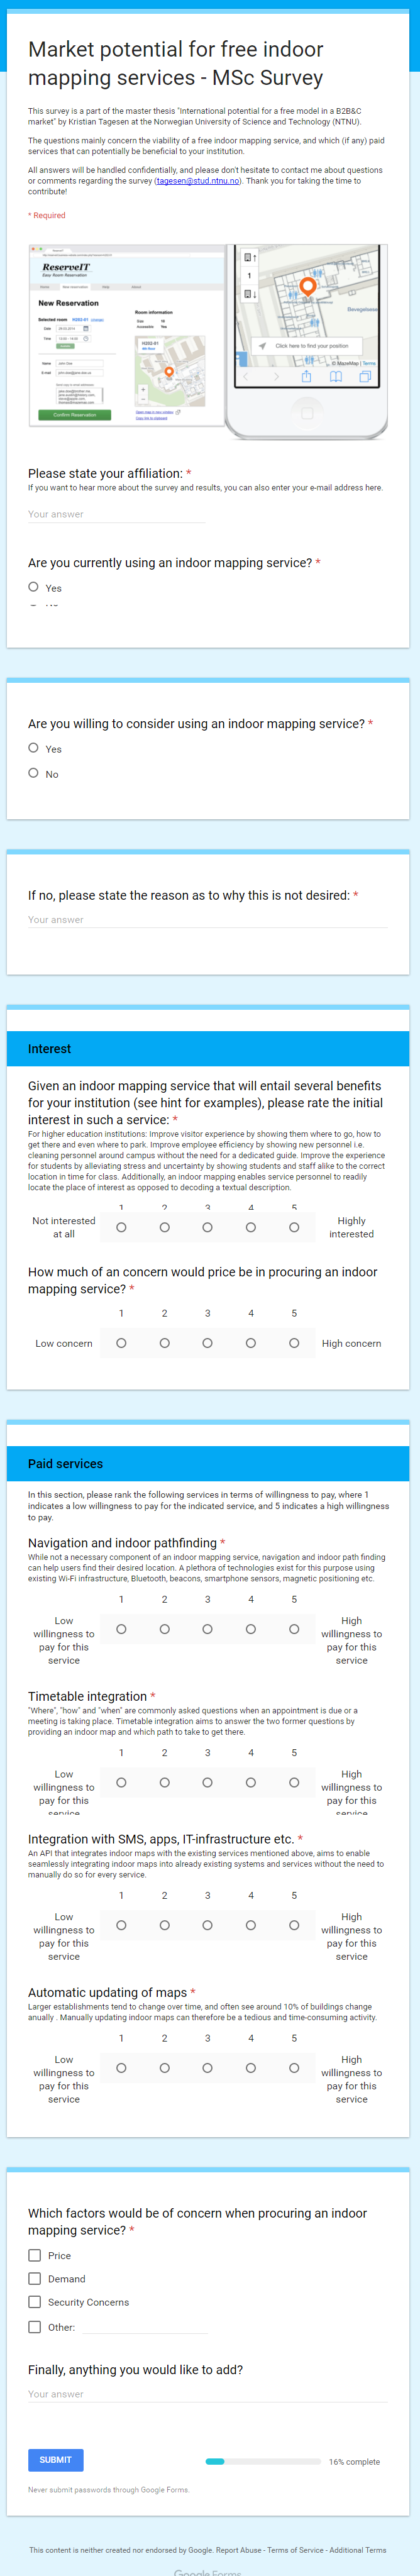
\includegraphics[width=\textwidth]{figs/survey.png}}
    \caption{Screenshot of the international research survey response form, part 1}
    \label{fig:s1}
\end{figure}

\begin{figure}[H]
    \centering
    \fbox{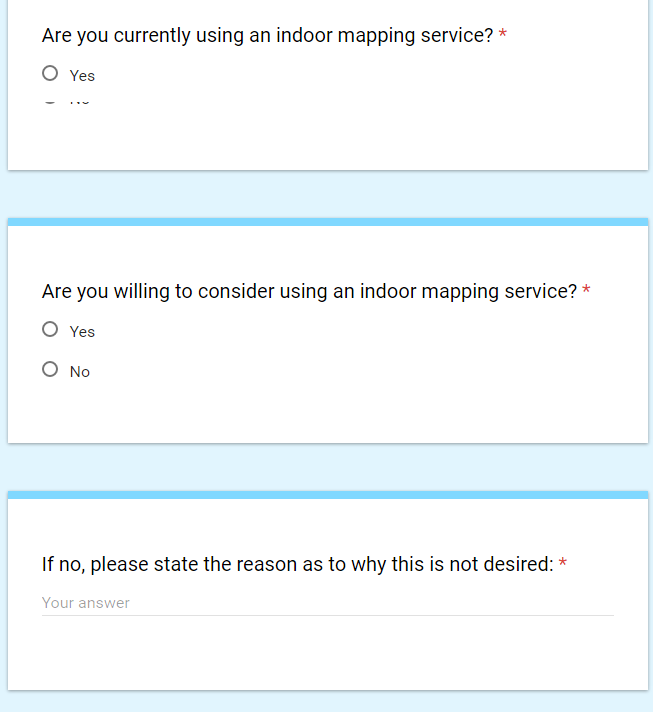
\includegraphics[width=\textwidth]{figs/s2.png}}
    \caption{Screenshot of the international research survey response form, part 2}
    \label{fig:s2}
\end{figure}

\begin{figure}[H]
    \centering
    \fbox{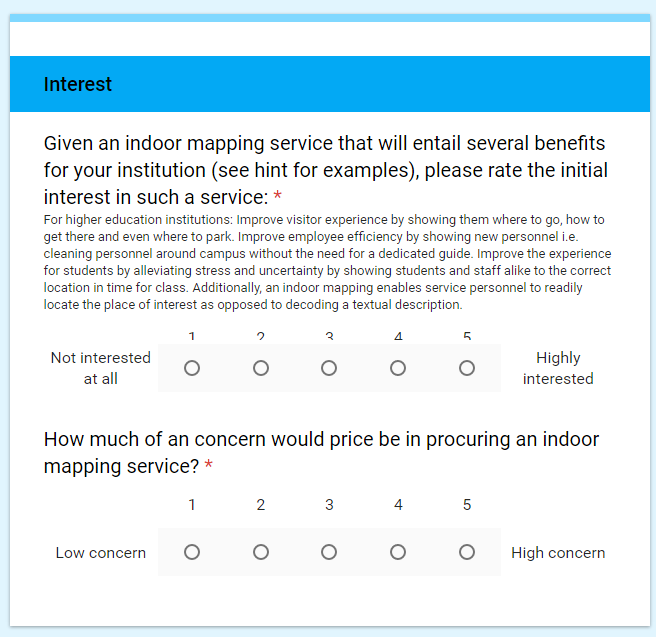
\includegraphics[width=\textwidth]{figs/s3.png}}
    \caption{Screenshot of the international research survey response form, part 3}
    \label{fig:s3}
\end{figure}

\begin{figure}[H]
    \centering
    \fbox{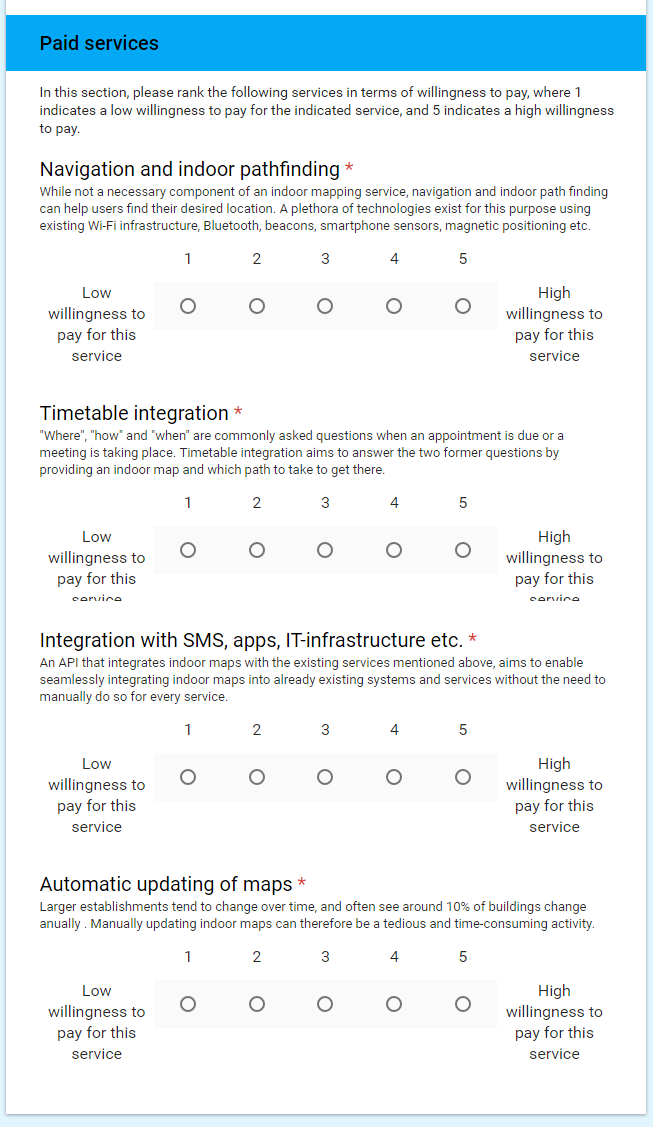
\includegraphics[width=\textwidth]{figs/s4.png}}
    \caption{Screenshot of the international research survey response form, part 4}
    \label{fig:s4}
\end{figure}

\begin{figure}[H]
    \centering
    \fbox{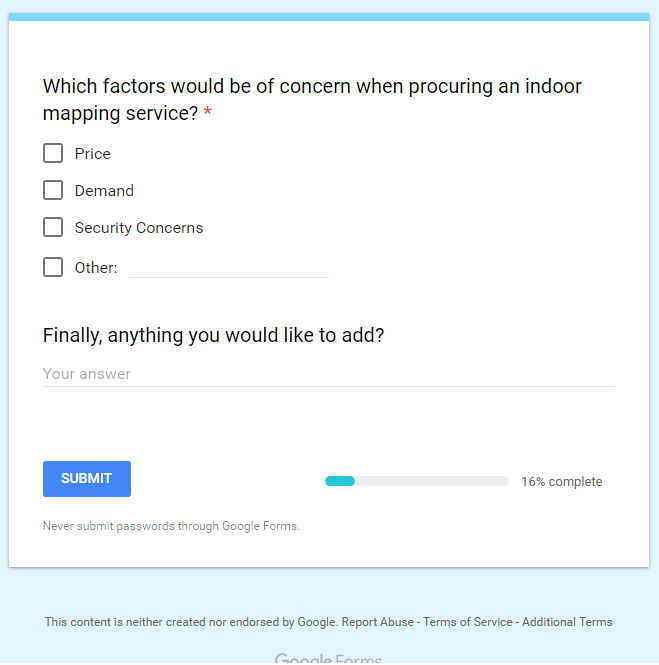
\includegraphics[width=\textwidth]{figs/s5.png}}
    \caption{Screenshot of the international research survey response form, part 5}
    \label{fig:s5}
\end{figure}

\chapter{An Introduction to the Business Model Canvas Framework}

This chapter introduces the reader to the framework that is Business Model Canvas, used to describe the proposed business model in Chapter 6. This particular framework has its merits in that it is used to invent, challenge and describe a business model \cite{strategyzer2016}. Further advantages include that it strips away any superfluous elements, improving its readability and enables users and business owners to focus on the most vital elements of a business model. It is also immensely flexible, as changes can be readily made without changing everything thanks to its modular design \cite{osterwalder2013business}. 


\begin{table}[H]
\centering
\caption{Building blocks of the Business Model Canvas}
\label{tab:canvas}
\begin{tabular}{|l|l|}
\hline
\textbf{Product}                                    & Value proposition     \\ \hline
\multirow{3}{*}{\textbf{Customer interface}}        & Customer segments     \\ \cline{2-2} 
                                                    & Relationship          \\ \cline{2-2} 
                                                    & Distribution channels \\ \hline
\multirow{2}{*}{\textbf{Financial aspects}}         & Cost structure        \\ \cline{2-2} 
                                                    & Revenue stream        \\ \hline
\multirow{3}{*}{\textbf{Infrastructure management}} & Key partnerships      \\ \cline{2-2} 
                                                    & Key activities        \\ \cline{2-2} 
                                                    & Key resources         \\ \hline
\end{tabular}
\end{table}

The framework consists of nine building blocks with varying degrees of importance, but an important relationship between them. When all building blocks are determined, they make up the total strategy of how a business would operate, make money and if desired, capture market shares. Table~\ref{tab:canvas} shows the different building blocks by their respective categories, and Figure~\ref{fig:businessmodelcanvas} shows the empty template for setting up the business model. The business model canvas is described here, as it will serve as a template for the proposal of the business model. Below follows a step-by-step description of the respective building blocks.


\section{Customer segments}
This building block consists of the different customer segments a company wishes to concentrate on and reach out to. A market may be single or multi-sided, containing at a minimum a segment per market side. Media companies, credit card companies and to some extent social networking sites among others fall into a multi-sided market category. It is important to note that when offering a value proposition to a market, market size is an important factor, as smaller, niche markets may be a viable market segment as opposed to a bigger market. Finally, diversified products offered through the value proposition may be used to reach smaller subsets of the market.

\section{Value proposition}
The value proposition is the building block that describes how a company is different from other competing companies. It details how a company's products or services can create value for their respective customer segments, where values may be qualitative or quantitative. Several means of creating value among customers  includes lower pricing (price-sensitive segments), design (aesthetically appealing products), status (well-known brands), customisation (tailor-made services or products) and performance-driven products. Additionally, introducing a brand new disruptive technology i.e. cell-phones may benefit a business' customer segment, even though it may initially be viewed as unnecessary. Offering consultancy services can also be a value proposition in itself, for instance IT-consultancy services. Concretely, in the framework one wishes to map a value proposition to a particular customer segment, in order to identify the needs of this particular segment.

\section{Distribution channels}
Distribution channels concerns how a value proposition is delivered to a customer segment. A channel serves multiple purposes, with the most important being raising awareness around the products or services a company is offering and aiding customers in understanding the value propositions. It also serves a perhaps equally important function in allowing for products or services to be purchased. Furthermore, the channels can be broken into different phases, depending on what phase a product is in. These include:

\begin{itemize}
    \item \textbf{Awareness}: Raising awareness among customers.
    \item \textbf{Evaluation}: How customers are able to evaluate the value proposition.
    \item \textbf{Purchase}: How products are purchasable from the customer's point of view.
    \item \textbf{Delivery}: How a value proposition is delivered to a customer.
    \item \textbf{After sales}: How on-going customer support is handled post-purchase.
\end{itemize}
Along with the next block, Customer relationships, the channels block forms how a business interfaces with their customers. 

\section{Customer relationships}
The different types of relationships a business establishes with their respective customer segments are detailed in the customer relationships block. From a business' perspective, having good customer relationships may entail several benefits in increasing their sales volume, gaining new customers and keeping their existing customers from leaving. The perhaps simplest relationship between a business and a customer lies in personal assistance, where actual, dedicated personnel from the business side is serving any customer need from any part of the sales cycle. In a \gls{b2b} market one may have one dedicated person or team per customer, while in a \gls{b2c} market this might not be manageable and call centres or e-mail respondents serves the purpose better. On the flipside, having customers manage themselves entirely either through robust online self-services or inter-customer relationships is also an option depending on the product or service provided. Lastly, co-creation where companies and customers share responsibility for the product is a modern take on a customer relationship, seen in social networks and user-creation oriented services i.e. YouTube.

\section{Revenue streams}
How much cash-flow each customer segment generates constitutes the revenue stream building block. It is essential for the profitability of a product or service, with revenue streams being either a one-time fee or recurring payments. Several ways to generate revenue streams include:

\begin{itemize}
    \item \textbf{Subscription fees: }By selling a service, a business may charge its customers of that service for any given time period. 
    \item \textbf{Licensing: }In companies where some form of intellectual property is made, it is possible to generate revenue by the sales or lending of these properties.
    \item \textbf{Advertising: }This type of revenue stream is generated from advertising a product or service on the behalf of some other business entity.
    \item \textbf{Brokerage fees: }By providing services between two parties and taking a fee for the transactions that take place.
    \item \textbf{Asset sale: }Selling the rights to one instance of a product falls into this category, and is the most traditional way of exchanging goods.
\end{itemize}

At this point of setting up the model, the customer segments are linked to its respective value propositions. Each of these should at this point be linked with a revenue stream.

\section{Key activities}
The key activities are the detrimental matters that a business needs to attend in order to deliver its value propositions. Together with key resources they are vital in creating and offering the value proposition to the customers, earning revenues and keeping customers satisfied. Consultant and service-oriented businesses often revolve around problem solving as a key activity, helping others with new and existing problems. For manufacturing companies and businesses, proposing, making and delivering products is a key activity, while software and banking service businesses may have a robust platform they offer their customers. In the case of the latter, the platform itself is the main component of their key activities. Lastly, it is important to connect the key activities to the value propositions, as the key activities are the main drivers of the value propositions.

\section{Key resources}
The key resources in this framework is absolutely vital for businesses in order to provide and create value propositions for its customers. Together with the key activities, they enable the generation of revenues, maintaining customer relationships and reach markets. Several types of key resources include:  physical (buildings, manufacturing plants), human (consultancy and r\&d services), financial (gaining and edge on competitors by lowering the price point) and intellectual (intellectual properties, brands etc.). The goal 
of the key resources is for the business to surpass competitors on key areas of the key resources.

\section{Key partnerships}
This building block concerns the partnerships, suppliers and other third party entities needed to make the business model work. The partnerships can vary in nature, where competitors and non-competitors can forge alliances or creating joint ventures. Any non-in-house solutions have to be supplied by third parties be it manufacturing parts or personnel. Motivations for creating partnerships include optimising the allocation of resources, reducing risk and to cut down on activities not vital in delivering a final product or service. As such, key partnerships can be linked with activities that aren't necessarily key to drive a business' value proposition. 

\section{Cost structure}
Different cost structures include fixed costs, variable costs, economies of scope and economies of scale. Fixed costs are volume-independent, and is usually examples of employee salary, rental costs and other facilities. Variable costs are volume-sensitive, while economies of scale concerns the costs changing as a result of a change in the scale of operation. Economies of scope on the other hand benefits businesses that diversify the number of different products or services offered, and is volume-insensitive in this regard. Different cost-structures exist in cost-driven and value-driven models. The former focuses on minimising the costs, and the latter model fits companies that less concerned with price and focuses more on value creation.
Lastly, it is important to note the relationship between cost structures and key activities, as the key activities drive a business' cost structures. 

\begin{figure}[]
    \centering
    \includegraphics[width=10cm]{figs/busmodcanvas.png}
    \caption{Business Model Canvas template. \textcopyright businessmodelgeneration.com}
    \label{fig:businessmodelcanvas}
\end{figure}

\end{document} 
